\documentclass[a4paper,12pt]{article}

\usepackage[utf8]{inputenc}
\usepackage{amsmath, amssymb}
\usepackage{graphicx}
\usepackage{float}
\usepackage{caption}
\usepackage{geometry}
\usepackage{hyperref}
\usepackage{enumitem}
\usepackage{textcomp}

\geometry{a4paper, margin=1in}

\title{Laborbericht: Messtechnik und Fehlerrechnung}
\author{Helen Klos \\Matrikelnummer: 2222449 \\ \\Sandro Fahrion \\Matrikelnummer: 6684592}
\date{29.-30.10.2024}

\begin{document}
\hyphenpenalty=1000
\exhyphenpenalty=1000
\sloppy
\setlength{\emergencystretch}{5pt}
\maketitle

\begin{figure}[H]
    \centering
    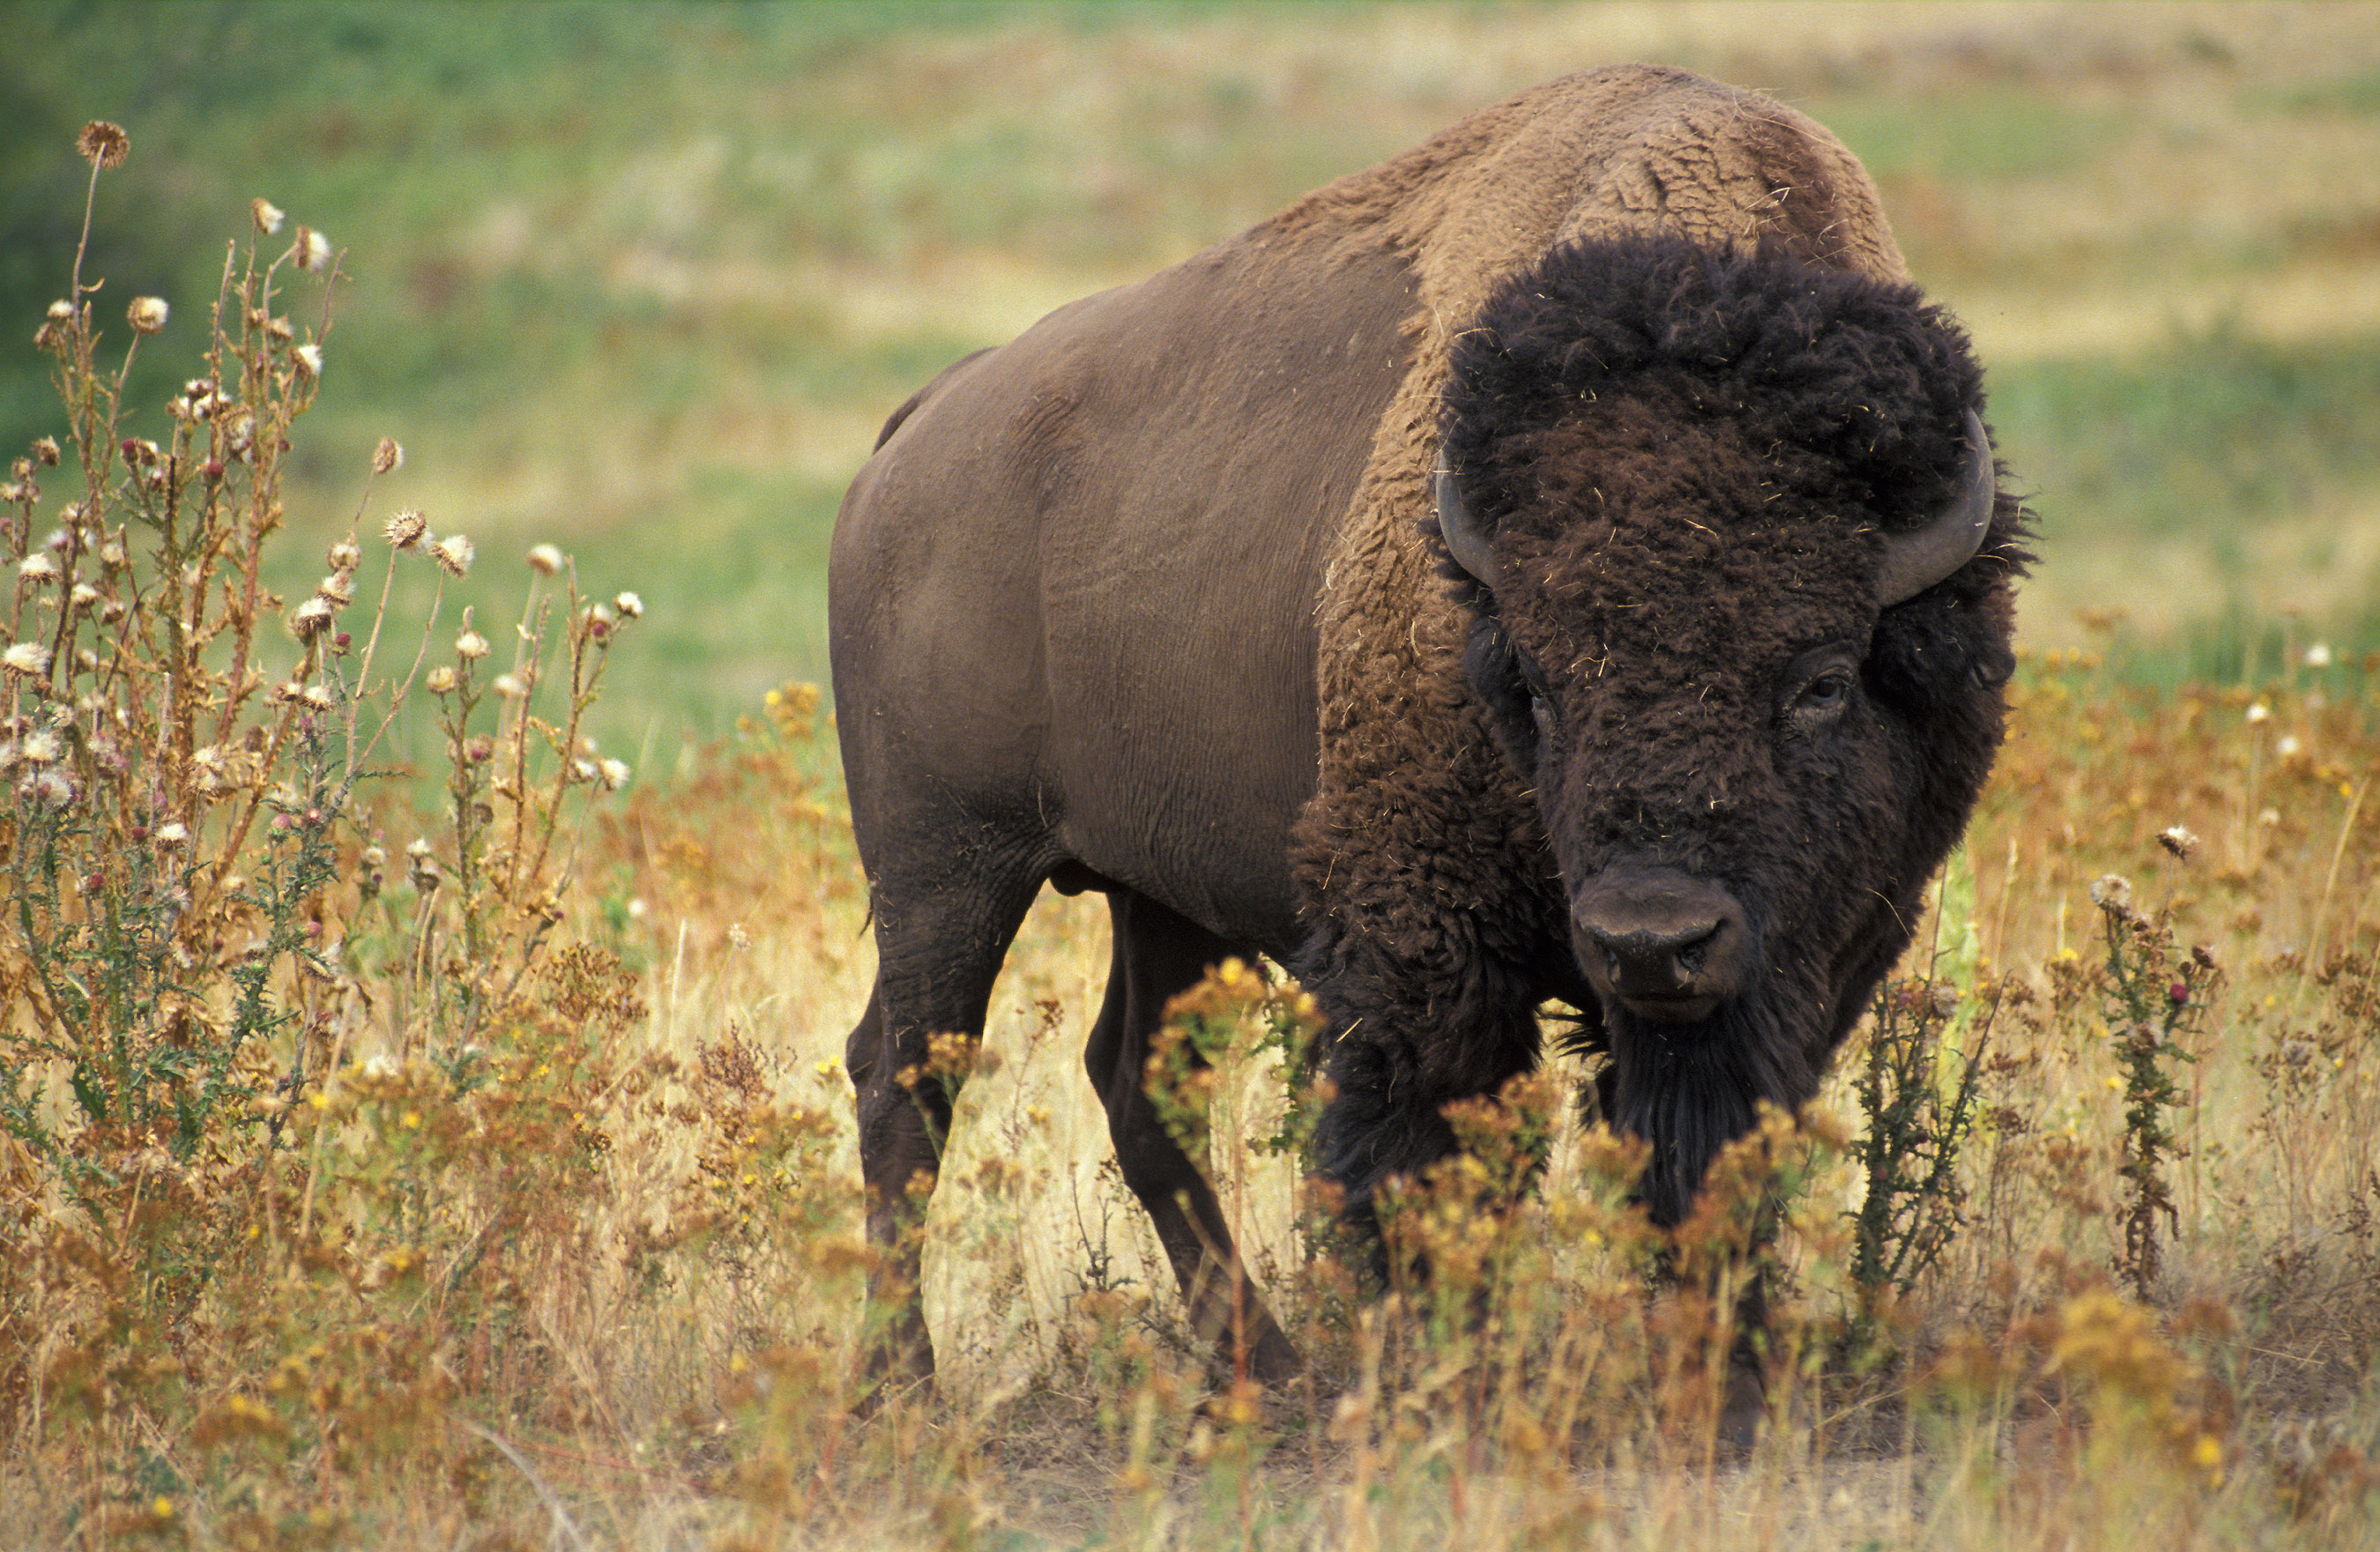
\includegraphics[width=1.0\textwidth]{../Quellen/Labor2/Titelbild.jpg}
\end{figure}
\newpage
\tableofcontents
\newpage

\section*{Einführung und Überblick}
\addcontentsline{toc}{section}{Einführung und Überblick}
Die moderne Messtechnik bildet die Grundlage zahlreicher technischer sowie naturwissenschaftlicher Erkenntnisse. Allerdings ist zu berücksichtigen, dass Messergebnisse niemals vollständig fehlerfrei sind. Die Ursachen für Messfehler und -ungenauigkeiten sind vielfältig. Als Ursachen für Messfehler und -ungenauigkeiten können beispielsweise eine fehlende Kalibrierung, Linearität und Stabilität der verwendeten Messinstrumente oder eine mangelnde Qualität des Messobjekts genannt werden. Des Weiteren kann auch der*die Messende selbst als Ursache in Betracht gezogen werden, welcher, zum Beispiel durch eine mögliche Sehschwäche oder einen ungünstigen Winkel, die Messwerte ungenau abliest. Nicht angepasste oder unvollkommene Messmethoden können ebenfalls zu einer Verfälschung der Messung führen.\\
Genannte Ursachen können zu drei verschiedenen Fehlerarten führen: grobe, statistische und systematische Fehler. \\

\noindent In diesem Laborbericht werden Versuche beschrieben, welche die Genauigkeit verschiedener Bauteile ermitteln. Des Weiteren beschäftigen sich diese mit Fehlerrechnung



\newpage

\section{Versuch 1: Kapazitätsmessung eines unbekannten Kondensators (Black Box)}

\subsection{Zielsetzung}
Das Ziel des ersten Versuchs bestand darin, die Kapazität eines unbekannten Kondesators in einer Black-Box zu bestimmen. 

\subsection{Bauteile und Messgeräte}
\subsubsection*{Messgeräte}
\begin{itemize}
\item Teledyne Technologies Funktionsgenerator T3AFG80 80 MHz
\item Keysight Oszilloskop (DSOX1102A)
\item Fluke 87 V True RMS Multimeter
\item Oszilloskop BNC Tastkopf mit Messklemme
\item Steckkabel (mehrere)
\item Tru Components Steckbrett
\item Bananenkabel (schwarz und rot)
\item Sicherheits-Klemmprüfspitze (2 Stück)
\end{itemize}

\subsubsection*{Bauteile}
\begin{itemize}
\item Black-Box (Nr. 18-30)
\item Widerstand Nominalwert 4,7 k$\Omega$
\end{itemize}
\newpage

\subsection{Messkonzept}
Zu Beginn wurde die Formel der Ladekurve \( u\textsubscript{c} = U (1 -e ^{-\frac{t}{RC}}) \) und der Entladekurve  \( u\textsubscript{c} = Ue ^{-\frac{t}{RC}}) \) grafisch am Computer dargestellt (siehe Figure 1). 

\begin{figure}[H]
    \centering
    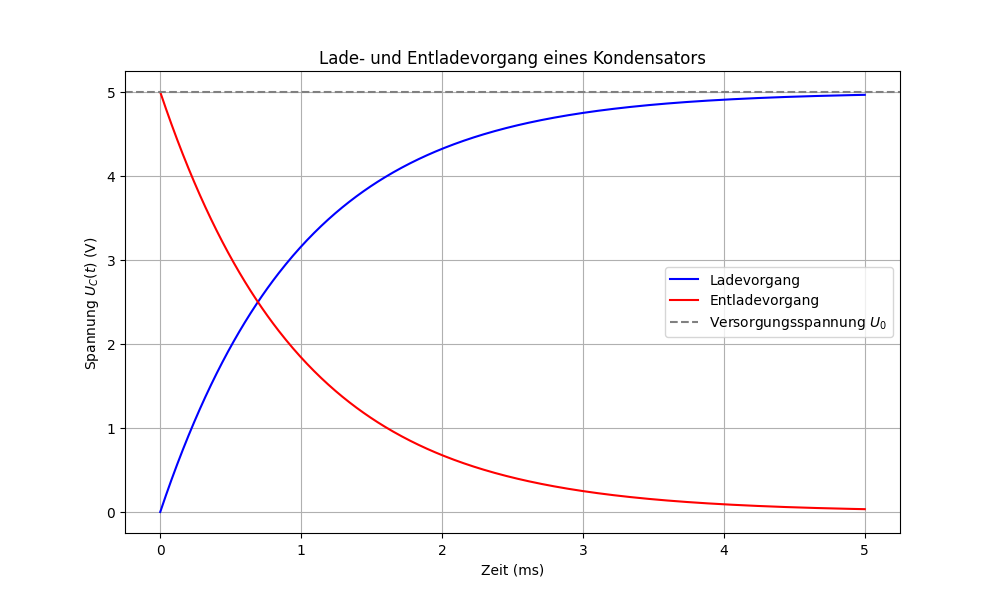
\includegraphics[width=1.0\textwidth]{../Quellen/Labor2/Lade-EntladefunktionSkizze.png}
\caption{Ladekurve (blau) und Entladekurve (rot) eines Kondensators}
\end{figure}

\noindent Diese sollte in den folgenden Schritten mit dem Oszilloskop sichtbar gemacht werden. Hierzu wurde sich zunächst überlegt, wie der Funktionsgenerator einzustellen ist. Diese Einstellungen sind Table 1 zu entnehmen. Für die verwendete Frequenz muss dabei gelten, dass...!!!, warum einstellungen so?

\begin{table}[H]
	\centering
	\begin{tabular}{|c|c|c|c|}
		\hline
		\textbf{Frequenz} & \textbf{Signalform} & \textbf{Amplitude} & \textbf{Offset}\\
		\hline
		500 Hz & Rechtecksignal & 5 V\textsubscript{pp} & 2.5 V\textsubscript{dc}\\
		\hline
	\end{tabular}
	\caption{Einstellungen des Funktionsgenerators}
\end{table}

\noindent Nachem der Funktionsgenerator korrekt eingestellt war, wurde die Schaltung  für die Messungen aufgebaut. Dabei wurde sich an der in Figure 2 dargestellten Skizze orientiert. Der, in der Skizze dargestellte, 50$\Omega$ Widerstand ist der Innenwiderstand des Funktionsgenerators. Dieser muss bei späteren Rechnungen berücksichtigt werden.\\

\begin{figure}[H]
    \centering
    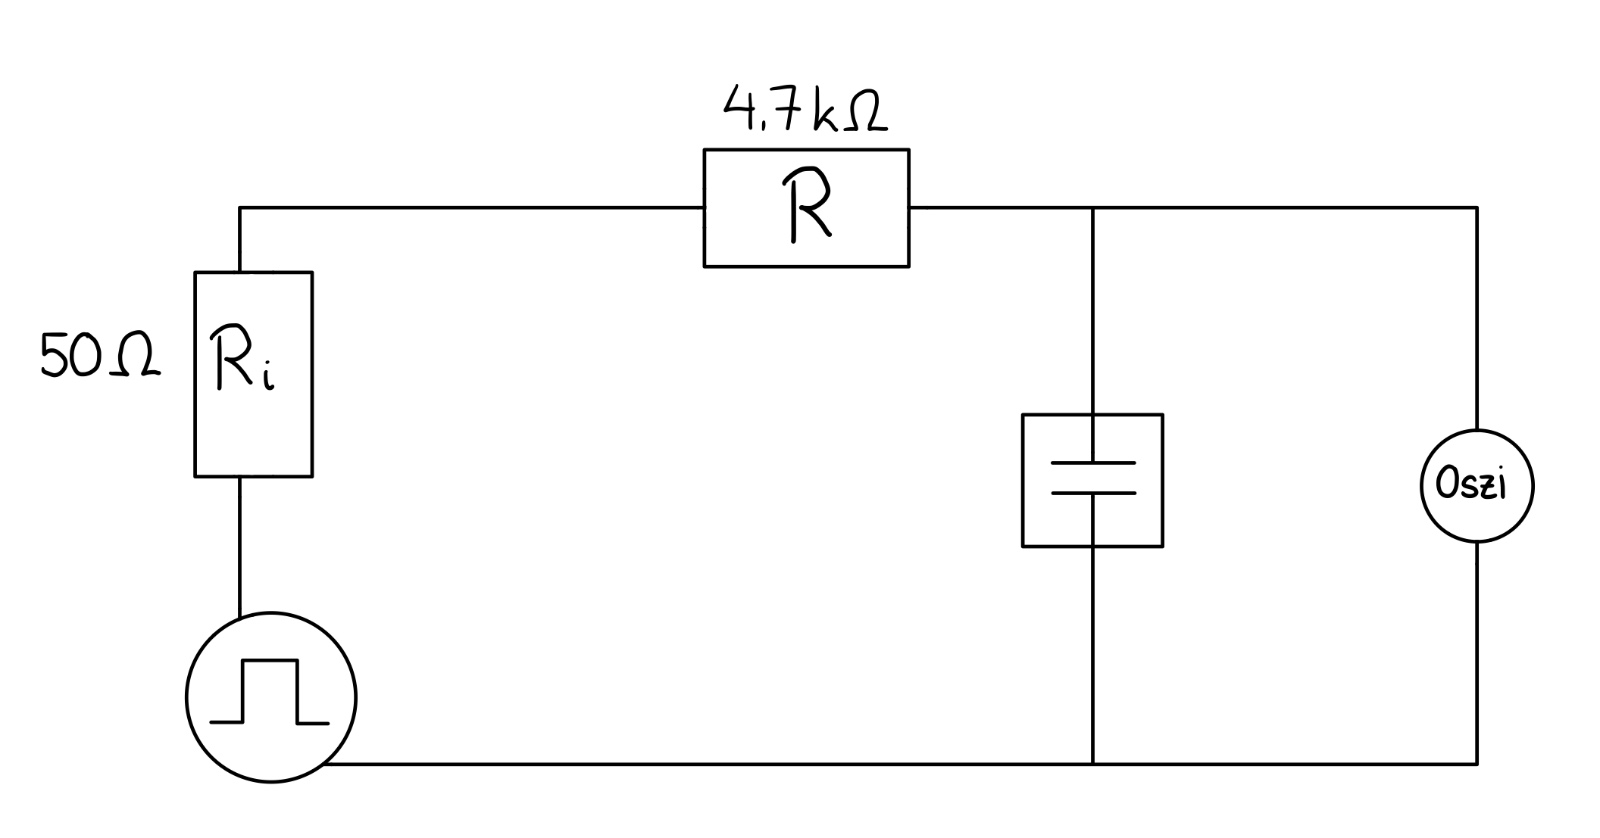
\includegraphics[width=0.6\textwidth]{../Quellen/Labor2/SchaltungsaufbauVersuch1.jpeg}
\caption{Schaltungsskizze}
\end{figure}

\noindent Für den Schatungsaufbau wurde zunächst der Funktionsgenerator mit einem ""kabel, mit Masse an die Black-Box und mit der Versorgungsspannung an das Steckbrett angeschlossen. An den Anschluss, an dem die Versorgungsspannung anliegt, wurde ein Steckkabel angeschlossen, welches dann den 4.7~$\Omega$ in Reihe schält. Die Black-Box wurde nun ebenfalls mit dem Steckbrett, hinter den Widerstand, verschaltet. Das Oszilloskop wurde nun parallel zur Black-Box angeschlossen. Hierfür wurde ein Oszilloskop BNC Tastkopf mit Messklemme verwendet. Die Masseklemme wurde an die Black-Box-Masse verbunden. Die Messklemme wurde mit einem weiteren Steckkabel am Steckbrett eingehakt, welches parallel zum Kondensator verläuft. Der Schaltungsaufbau ist in Figure 3 dargestellt.

\begin{figure}[H]
    \centering
    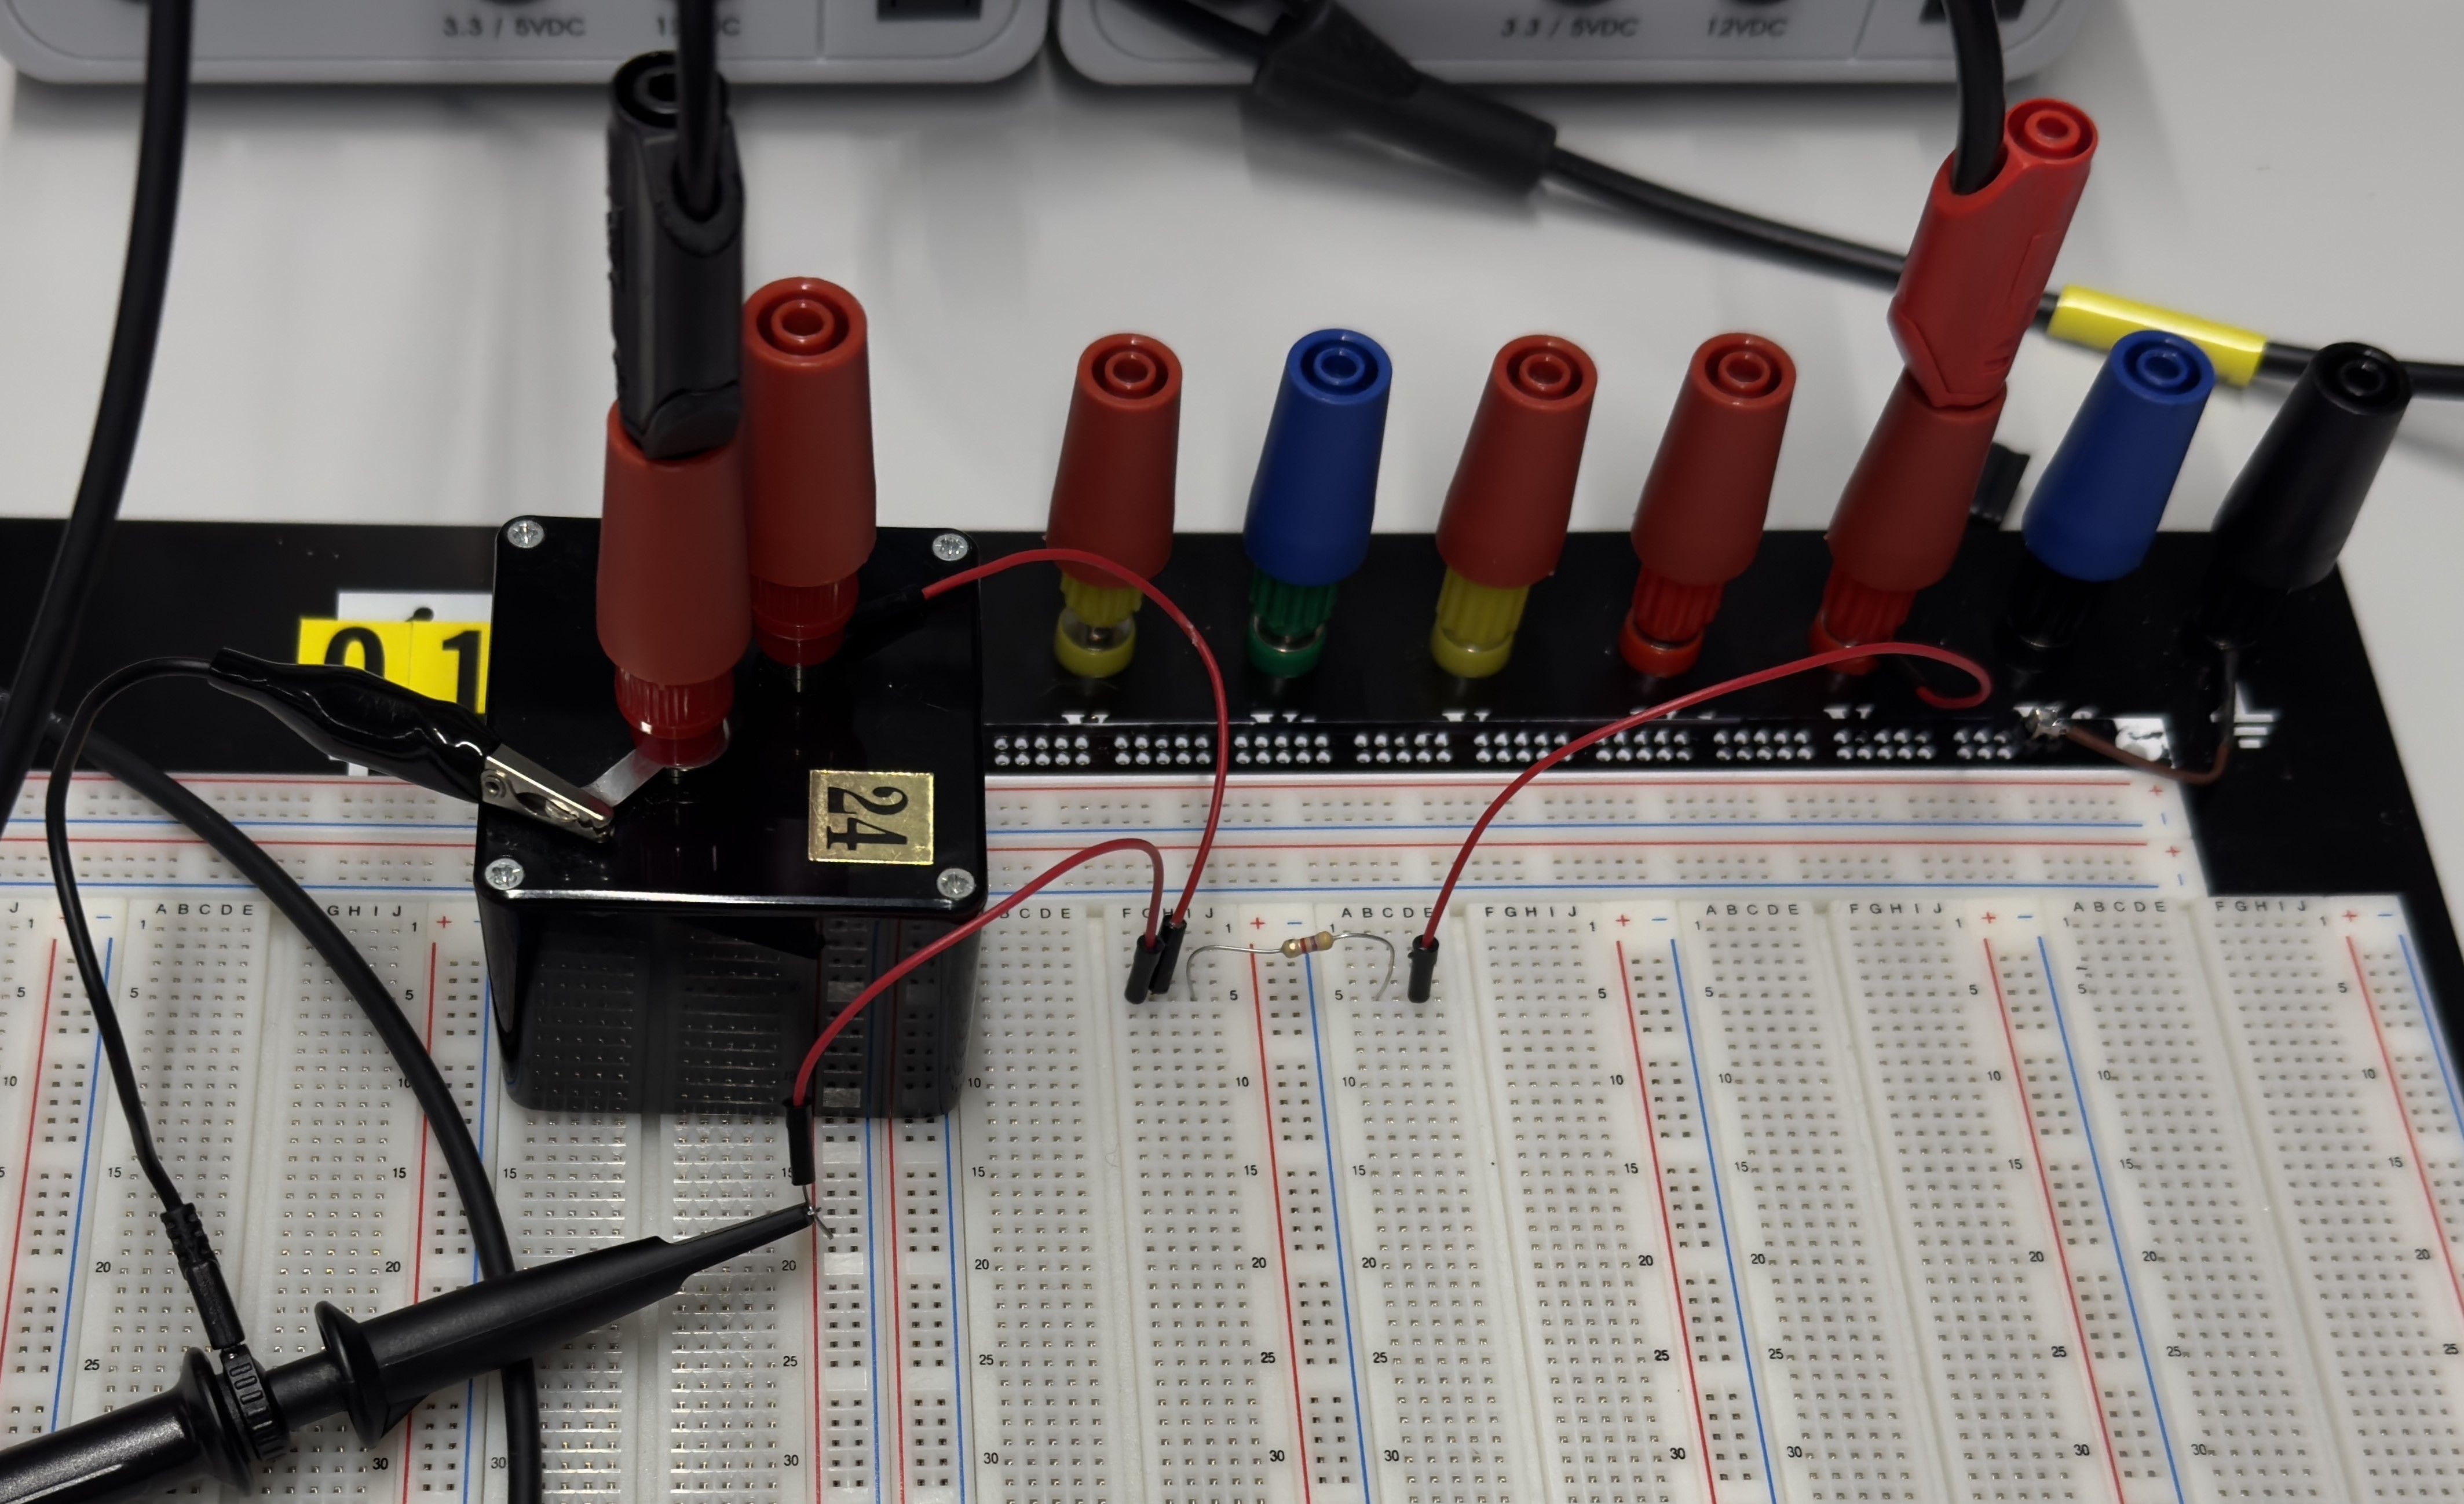
\includegraphics[width=0.8\textwidth]{../Quellen/Labor2/IMG_3965 - Kopie.jpeg}
\caption{Schaltungsaufbau}
\end{figure}

\noindent Der Verlauf der Lade- und der Entladekurve konnte nun am Oszilloskop abgelesen werden (siehe Figure 4). Diese wurde reingezoomt (siehe Figure 5), um die Zeitkonstante Tau ($\tau$) zu ermitteln. !!! \\
Anschließend an die Tau-Ermittlung sollte die Kapazität C\textsubscript{x} des Kondensators bestimmt werden. Hierzu wurde zuerst der ohm'sche Widerstand (4.7 k$\Omega$) mit dem Digital-Multimeter (DMM) nachgemessen. Der Widerstand wurde mit den Sicherheits-Klemmprüfspitzen, wie in Figure 6 gezeigt, gemessen. Mit diesem Widerstand, dem Innenwiderstand des Funktionsgenerators und der ermittelten Zeitkonstante konnte nun die Kapazität des Kondensators mit der Formel $\tau = R \cdot C$ ausgerechnet werden.

\[
C\textsubscript{x} ~=~ \frac{\tau}{R} ~=~ \frac{34.2 \cdot 10^{-6}s}{4611~\Omega + 50~\Omega} ~=~ 7337~pF
\]

\noindent In Table 2 sind alle in der Schaltung und der Messanordnung vorkommenden absoluten bzw. relativen Einzelfehler aufgelistet.!!!

\subsection{Messergebnisse}

\begin{figure}[H]
    \centering
    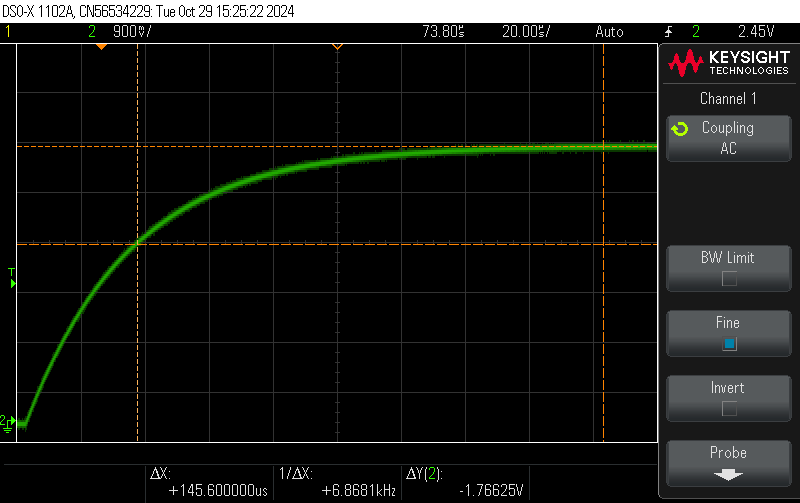
\includegraphics[width=0.8\textwidth]{../Quellen/Labor2/scope_0.png}
\caption{Ladekurve des Kondensators}
\end{figure}

\begin{figure}[H]
    \centering
    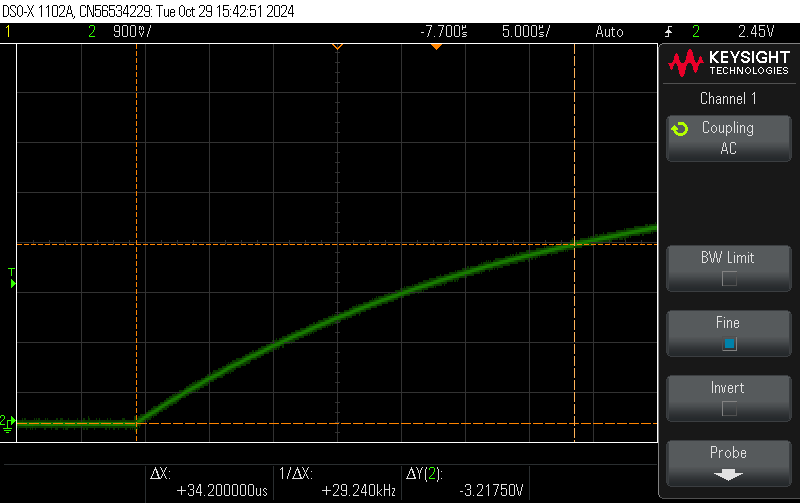
\includegraphics[width=0.8\textwidth]{../Quellen/Labor2/scope_1.png}
\caption{reingezoomte Ladekurve des Kondensators für Tau-Bestimmung}
\end{figure}

\begin{figure}[H]
    \centering
    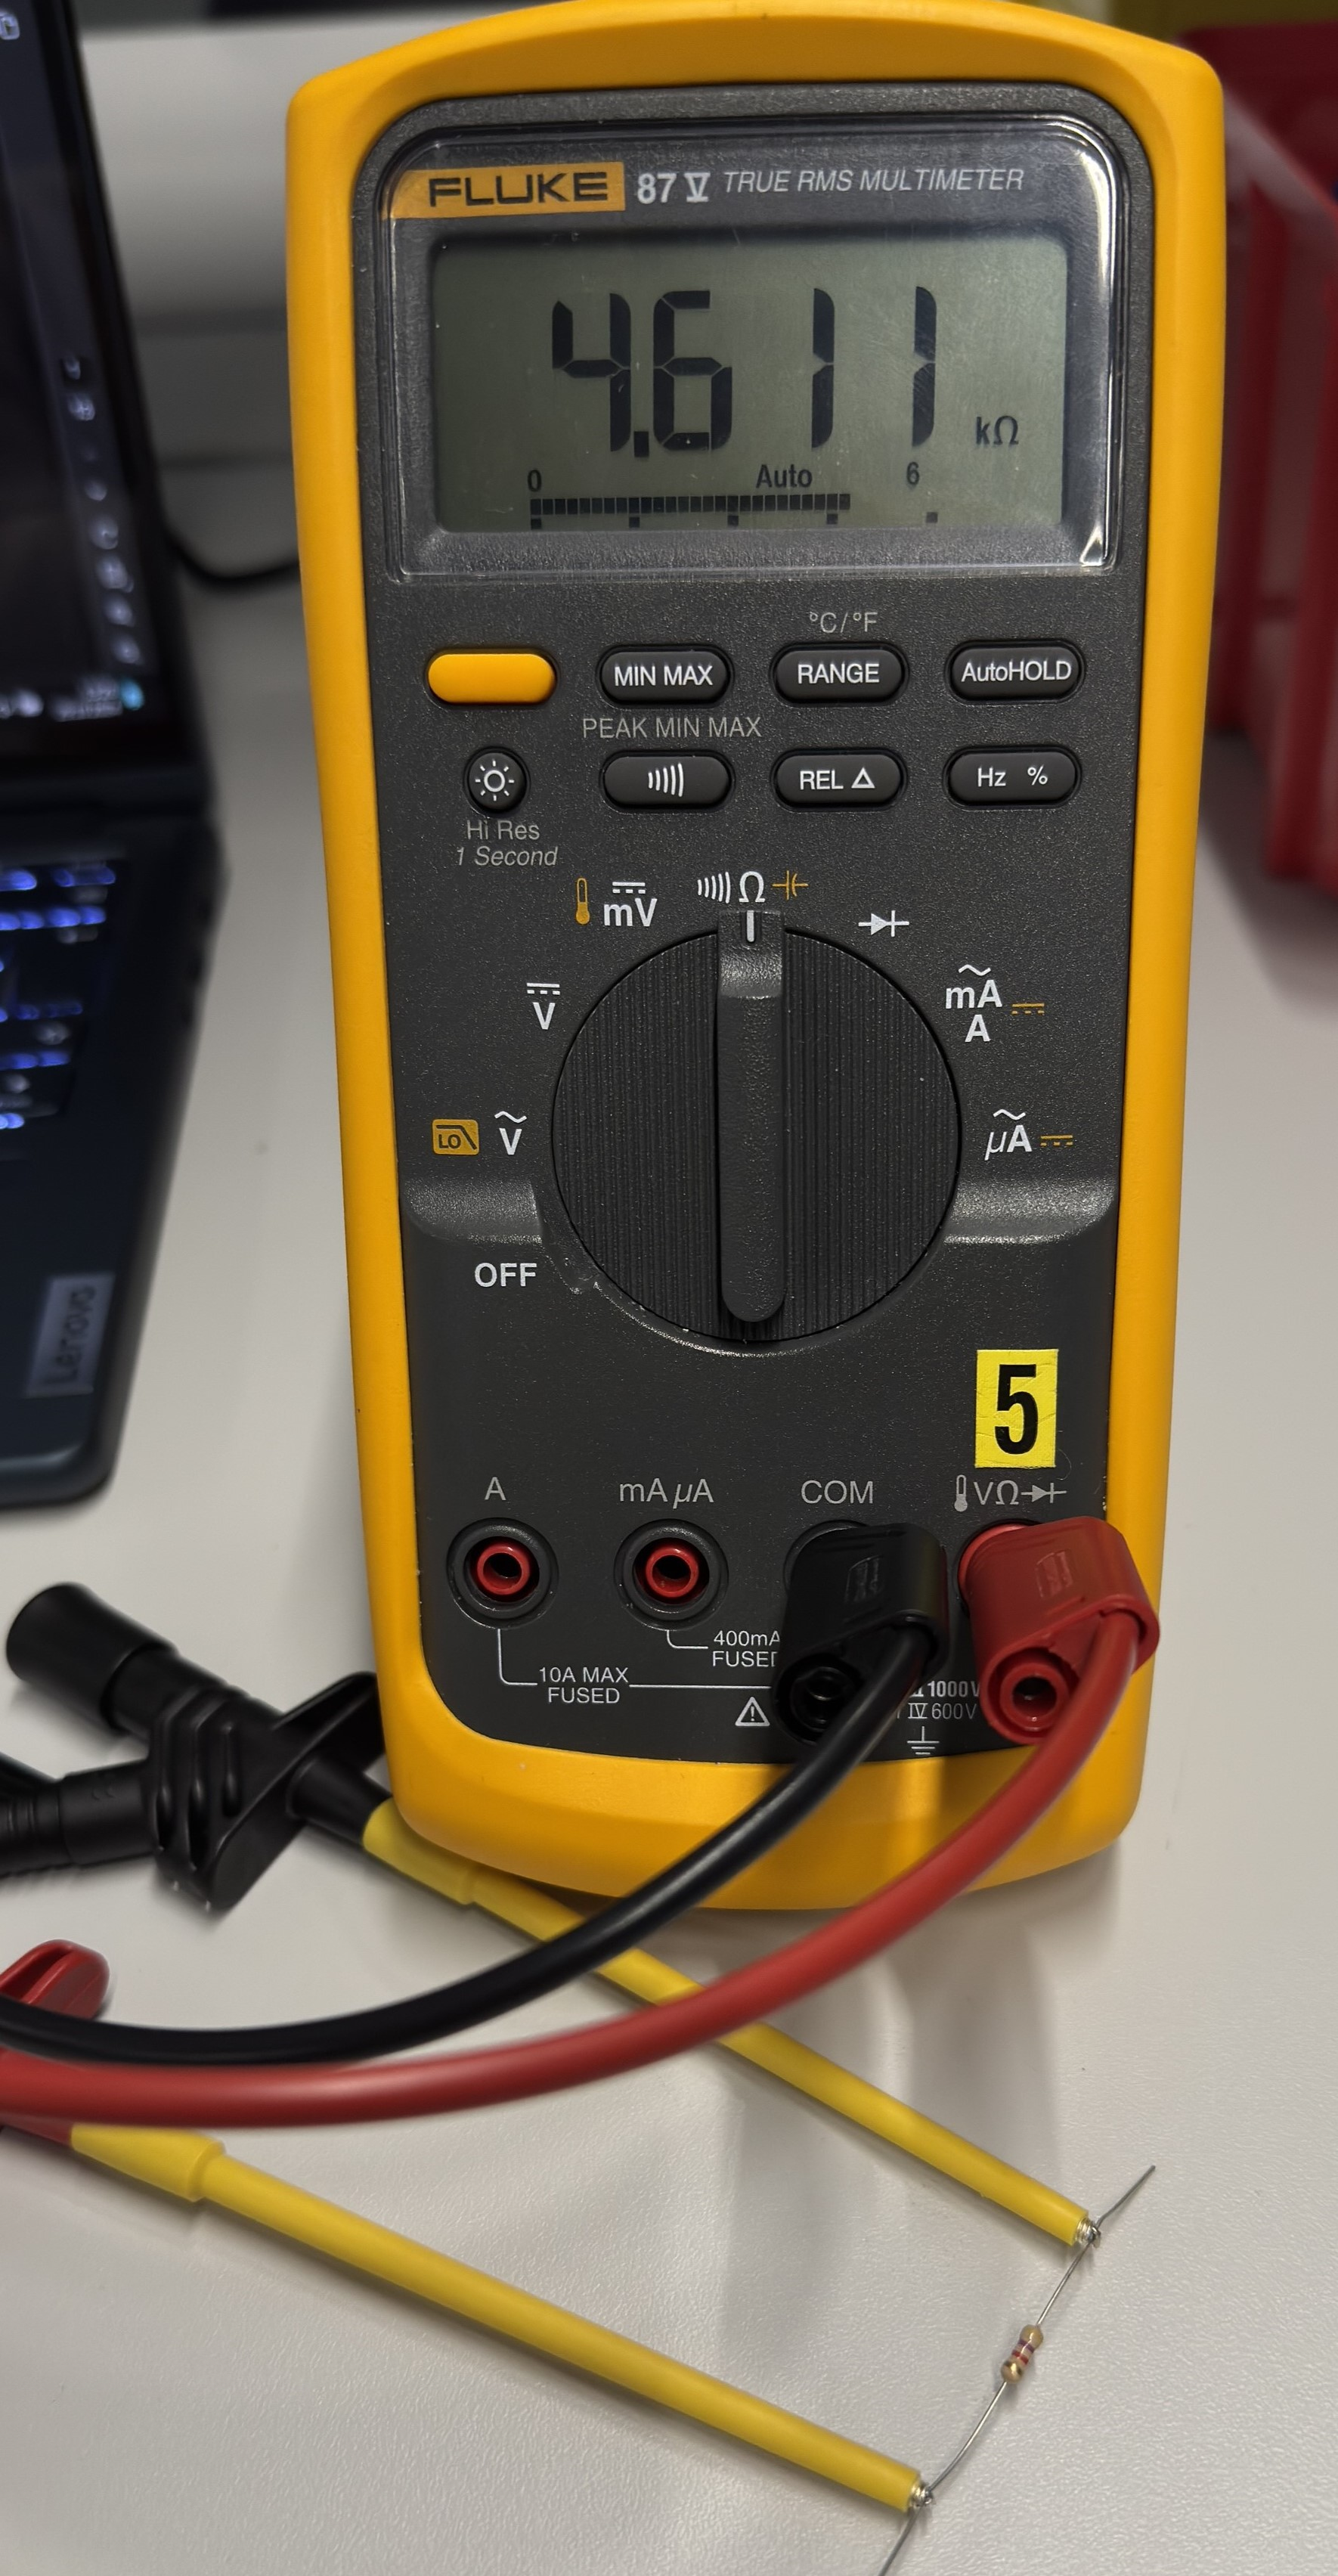
\includegraphics[width=0.5\textwidth]{../Quellen/Labor2/Fotos/IMG_3963gezoomt.jpeg}
\caption{Messung ohm'scher Widerstand mit dem DMM}
\end{figure}



\begin{table}[H]
	\centering
	\scalebox{0.8}{	
\begin{tabular}{|c|c|c|c|c|c|}
		\hline
		\textbf{Fehlerquelle} & \textbf{Einfluss} & \textbf{typische Größe} & \textbf{stat. oder sys.} & \textbf{Berücksichtigung?} & \textbf{relevant?}\\
		\hline
		R = 4.7 k$\Omega$ & DMM-Messung & \textperthousand ~siehe Datenblatt & statistisch & Fehlerrechnung & Ja\\
		\hline
		Oszilloskop & R\textsubscript{i},C\textsubscript{i} Tastkopf (10x) & 10 µ$\Omega$, $\sim$pF & systematisch & Nein \( < 0.5 \)\textperthousand & Nein\\
		  & x, y - Messung & \(\approx 3\) \% Datenblatt! & statistisch & Fehlerrechnung & Ja\\
		  & Curser & Steigung beachten & statistisch & Fehlerrechnung & Ja\\
		\hline
		Funktionsgenerator & Anstiegszeit & einige ns & systematisch & \( \approx 1 \) \textperthousand & Nein\\
		  & R\textsubscript{i} & 50 $\Omega$ & systematisch & Korrektur & Ja\\
		  &   & $\Delta R$\textsubscript{i} (\(\approx 1\)\%) & statistisch & 1$\%$ \( \Rightarrow\) $\pm ~0.5~\Omega$ & Nein\\
		  & Amplitude, Offset & - & systematisch & relativ & Nein\\
		\hline
		Kabel +5 V & Widerstand & \(\approx 20\)m$\Omega$ & systematisch & zu klein & Nein\\
		\hline
	\end{tabular}
	}
	\caption{}
\end{table}


\newpage
\section{Versuch 2: Passiver Zweipol (Black Box)}
\subsection{Zielsetzung}
Bestimmung der Bauteil-Typen (Möglichkeiten: R, L oder C) und deren Anordnung innerhalb einer
Black Box.

\subsection{Bauteile und Messgeräte}
\subsubsection*{Messgeräte}
\begin{itemize}
\item Teledyne Technologies Funktionsgenerator T3AFG80 80 MHz
\item Keysight Oszilloskop (DSOX1102A)
\item Netzgerät (NEP-8323)?
\item Fluke 87 V True RMS Multimeter
\item Oszilloskop BNC Tastkopf mit Messklemme
\item Steckkabel (mehrere)
\item Tru Components Steckbrett
\item Bananenkabel (schwarz und rot)
\item Sicherheits-Klemmprüfspitze (2 Stück)
\end{itemize}

\subsubsection*{Bauteile}
\begin{itemize}
\item Black-Box (Nr. 1-17)
\item Widerstand Nominalwert 4,7 k$\Omega$
\end{itemize}
\newpage

\subsection{Messkonzept}
Der Schaltungsaufbau des ersten Versuchs konnte so beibehalten werden. Es musste lediglich die Black-Box des ersten Versuchs durch eine Black-Box mit einer Nummer zwischen 1 und 17 ersetzt werden. In diesem Versuchsbericht wurde Nummer 6 verwendet. Diese konnte identisch zur vorherigen angeschlossen werden. Bevor die Schaltung aufgebaut wurde, wurde zunächst der Widerstand der verwendeten Black-Box mit dem DMM gemessen (siehe Figure 8). Nun wurde die Black-Box in die Schaltung integriert. Um herauszufinden, welche Bauteile sich in der Black-Box befinden und wie diese miteinander verschaltet sind, sollten die Frequenzen des Rechtecksignals verändert werden und dabei der Verlauf der Funktion auf dem Oszilloskop beobachtet werden. An dem Verlauf, welcher in Figure 9 zu sehen ist konnte mithilfe der Curser abgelsen werden, dass die Eingangsamplitude 5 V und die Ausgangsamplitude 2,96 V entspricht. Dazu kommt, dass es sich um ein periodisches Verhalten handelt und ein Lade- und ein Entladevorgang erkennbar sind. Daraus lies sich schließen, dass es sich in jedem Fall um einen Kondensator handeln muss. Da bei der Widerstands-Messung der Black-Box!!!

\begin{figure}[H]
    \centering
    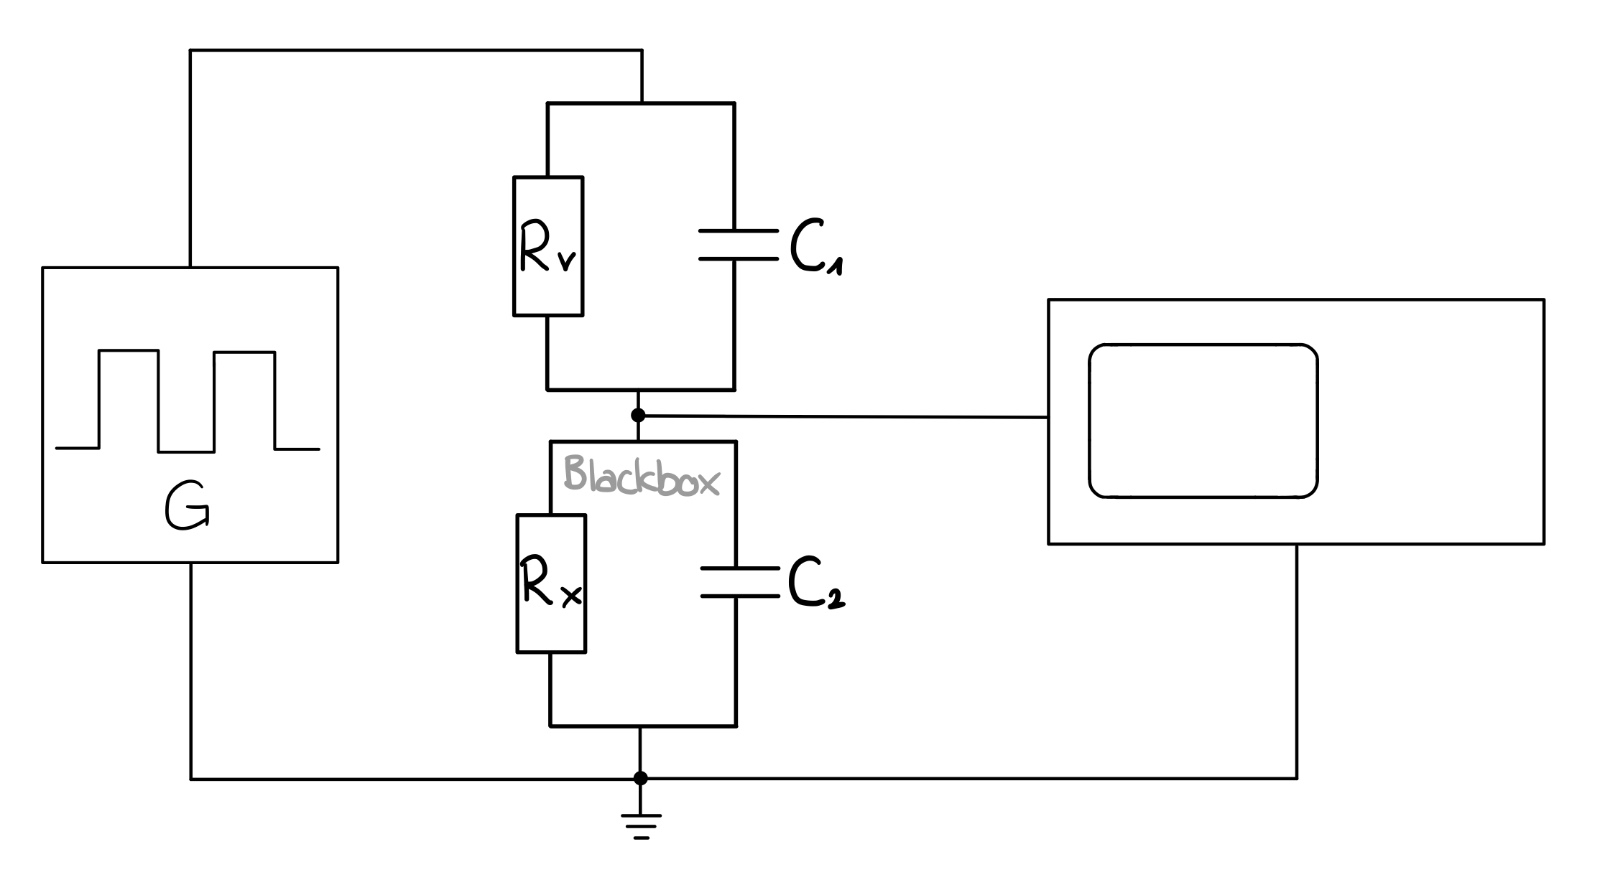
\includegraphics[width=0.8\textwidth]{../Quellen/Labor2/SkizzeVerschaltungWiderstandKondensatorVersuch2.jpeg}
\caption{Schaltskizze}
\end{figure}


\subsection{Messergebnisse}
\begin{figure}[H]
    \centering
    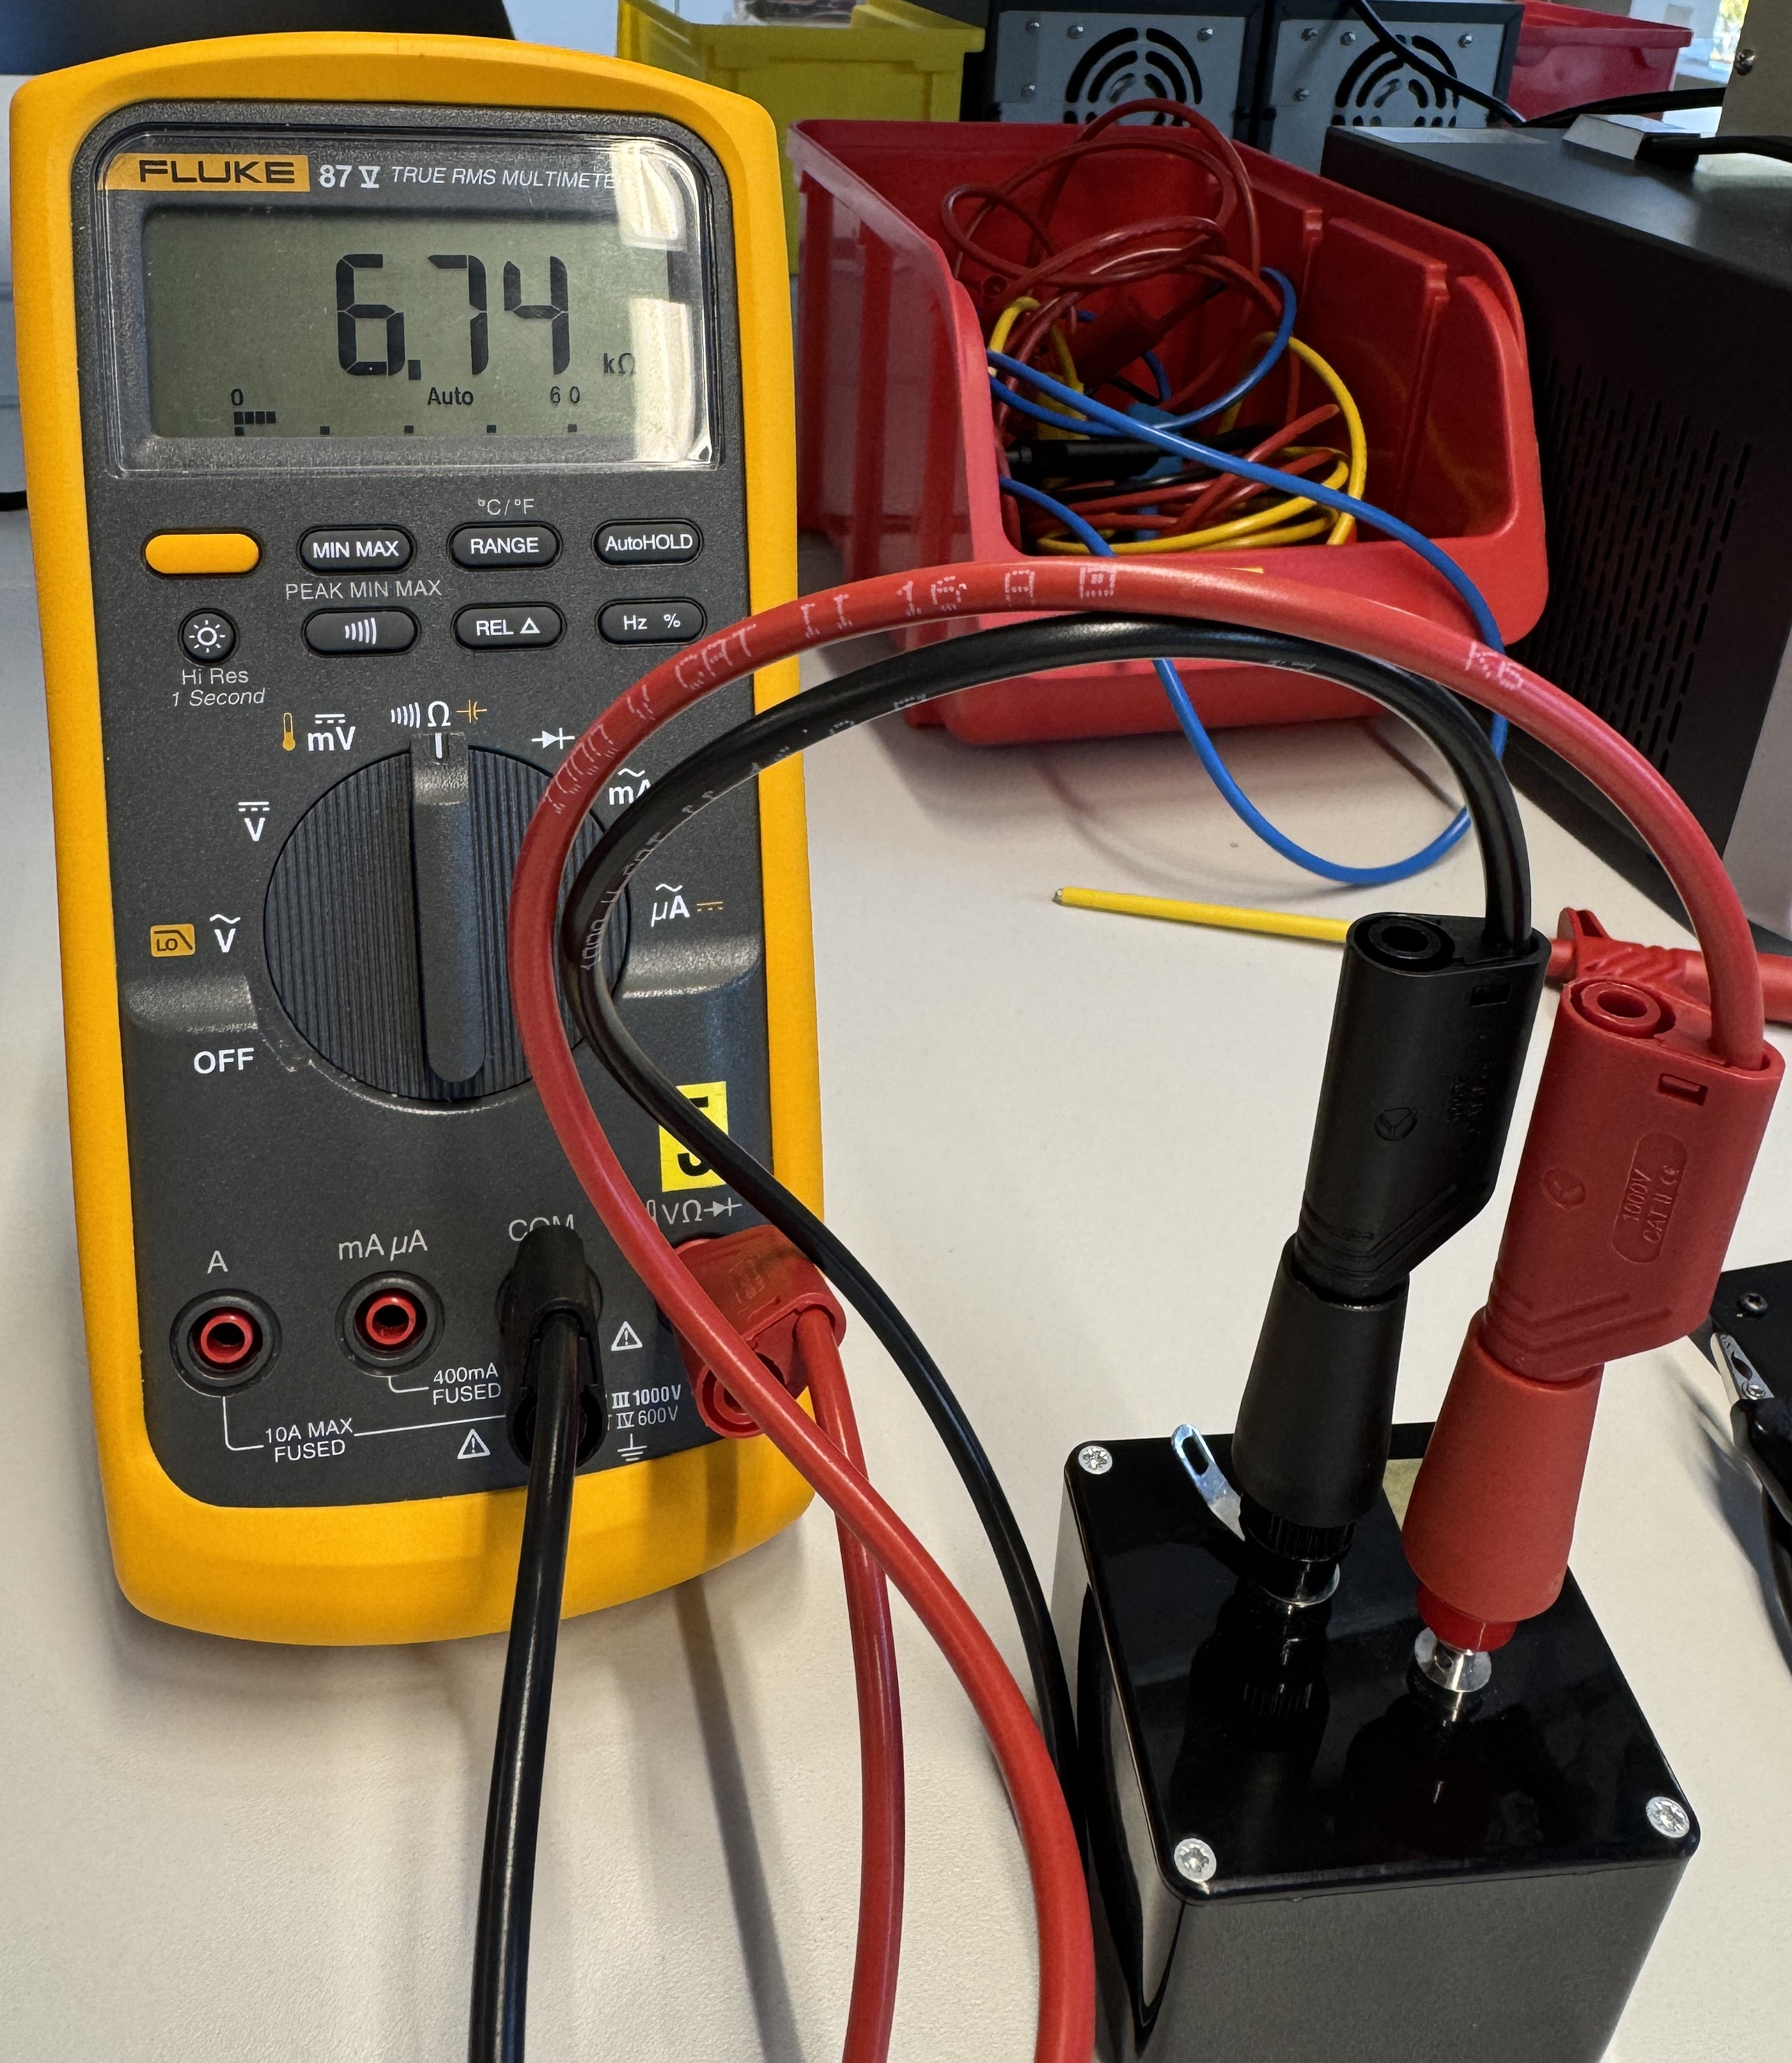
\includegraphics[width=0.5\textwidth]{../Quellen/Labor2/Fotos/IMG_3973gezoomt.jpeg}
\caption{...}
\end{figure}



\begin{figure}[H]
    \centering
    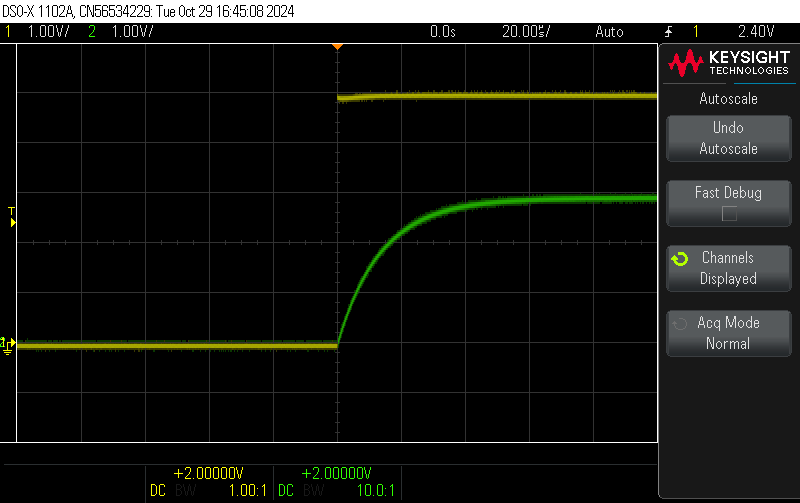
\includegraphics[width=0.8\textwidth]{../Quellen/Labor2/scope_3.png}
\caption{...}
\end{figure}





\newpage
\section{Versuch 3: Leistungsaufnahme eines elektrischen Widerstands}
\subsection{Zielsetzung}
Es soll die elektrische Leistung bestimmt werden, die bei Stromdurchfluss in
einem Widerstand R anfällt.

\subsection{Bauteile und Messgeräte}
\subsubsection*{Messgeräte}
\begin{itemize}
\item Netzgerät (NEP-8323)
\item Fluke 87 V True RMS Multimeter
\item Steckkabel (mehrere)
\item Tru Components Steckbrett
\item Bananenkabel (schwarz und rot)
\item Sicherheits-Klemmprüfspitze (2 Stück)
\end{itemize}

\subsubsection*{Bauteile}
\begin{itemize}
\item Widerstand Nominalwert 1 k$\Omega$ (2 Stück)
\end{itemize}
\newpage

\subsection{Messkonzept}
Zu Beginn dieses Versuchs, wurden die beiden Widerstände mit dem DMM nachgemessen (siehe Table 3), um die Genauigkeit der darauf folgenden Messungen zu steigern. Anschließend wurde das Netzgerät auf 5~V Spannung eingestellt und der Strom auf 200~mA begrenzt. Gemäß der Schaltskizze~1 (siehe Figure 10) wurde nun eine Schaltung aufgebaut (siehe Figure 11). Das Netzgerät versorgt das Steckbrett mit der voreingestellten Spannung. Der Strom wurde nun mit den Sicherheits-Prüfspitzen mittels direkter Strommessung auf 5.06~mA bestimmt (siehe Figure 11). Über die Formel \(P = I^2 \cdot R \) konnte nun die Leistung bestimmt werden.

\[
P ~=~ I^2 \cdot R ~=~ (5.06~mA)^2 \cdot 988~\Omega ~=~ 25.3~mW
\]\\

\noindent Messfehler!!!\\\\
Nun wurde die Versorgungsspannung auf 10~V erhöht. Die Schaltung wurde gemäß der Schaltskizze~2 (siehe Figure 10) umgebaut (siehe Figure 12). Nun sollte mit indirekter Strommessung gemäß der Formel \(P ~=~  (\frac{U}{R\textsubscript{v}})^2 \cdot R\) die Leistung bestimmt werden. Dabei soll r\textsubscript{v} als zweiter Widerstand!!!! dienen.

\[
P ~=~  (\frac{U}{R\textsubscript{v}})^2 \cdot R ~=~ (\frac{10~V}{996~\Omega})^2 \cdot 988~\Omega ~=~ 99.6~mW
\]

\noindent Messfehler!!!

\begin{figure}[H]
    \centering
    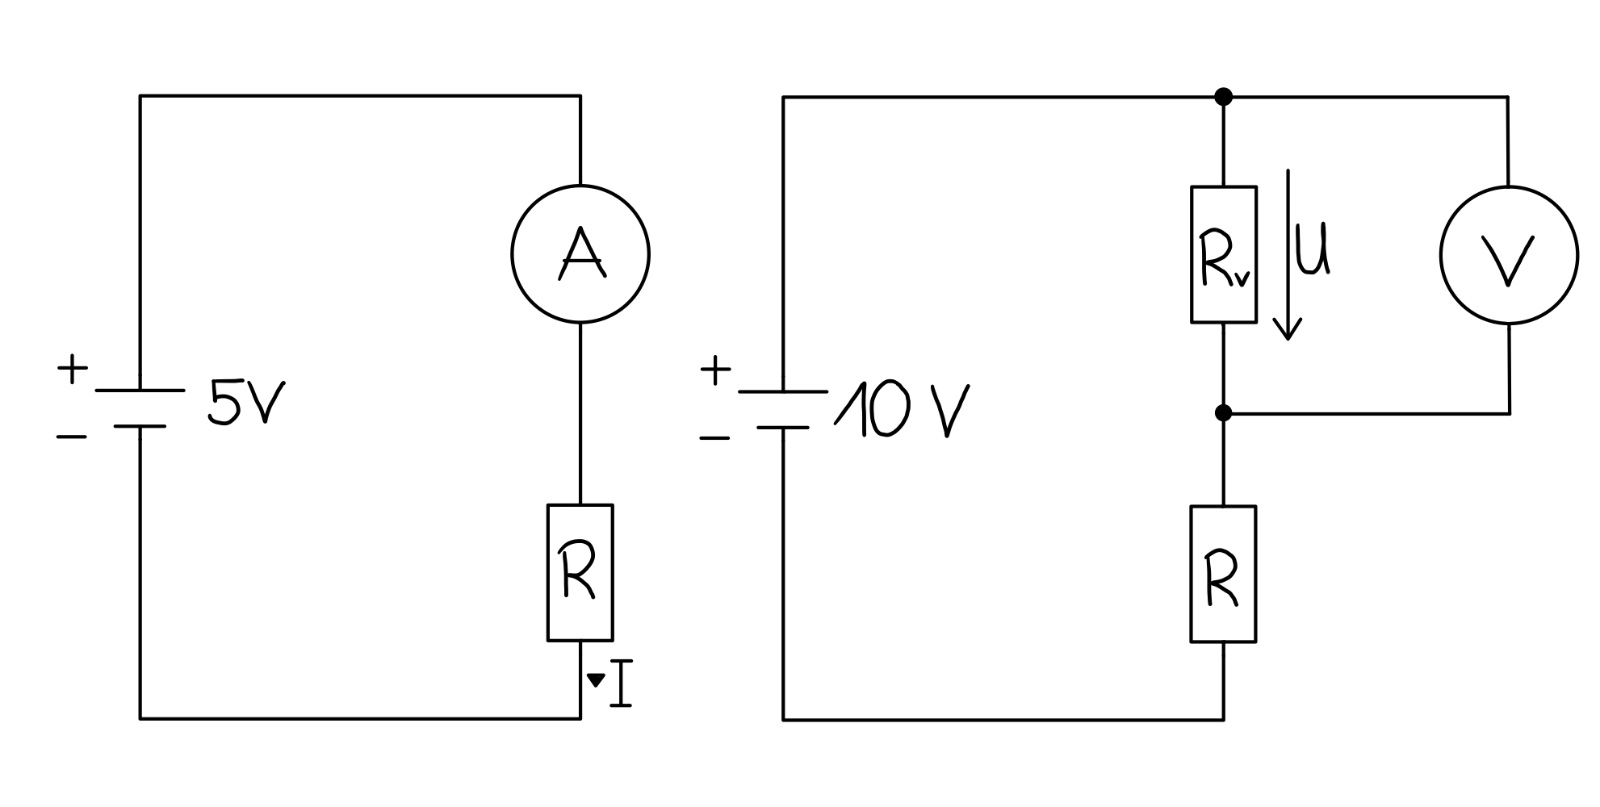
\includegraphics[width=0.8\textwidth]{../Quellen/Labor2/Schaltskizzen Widerstandsmessung.jpeg}
\caption{Schaltskizze 1 (Messung R) und Schaltskizze 2 (Messung R\textsubscript{v})}
\end{figure}



\begin{figure}[H]
    \centering
    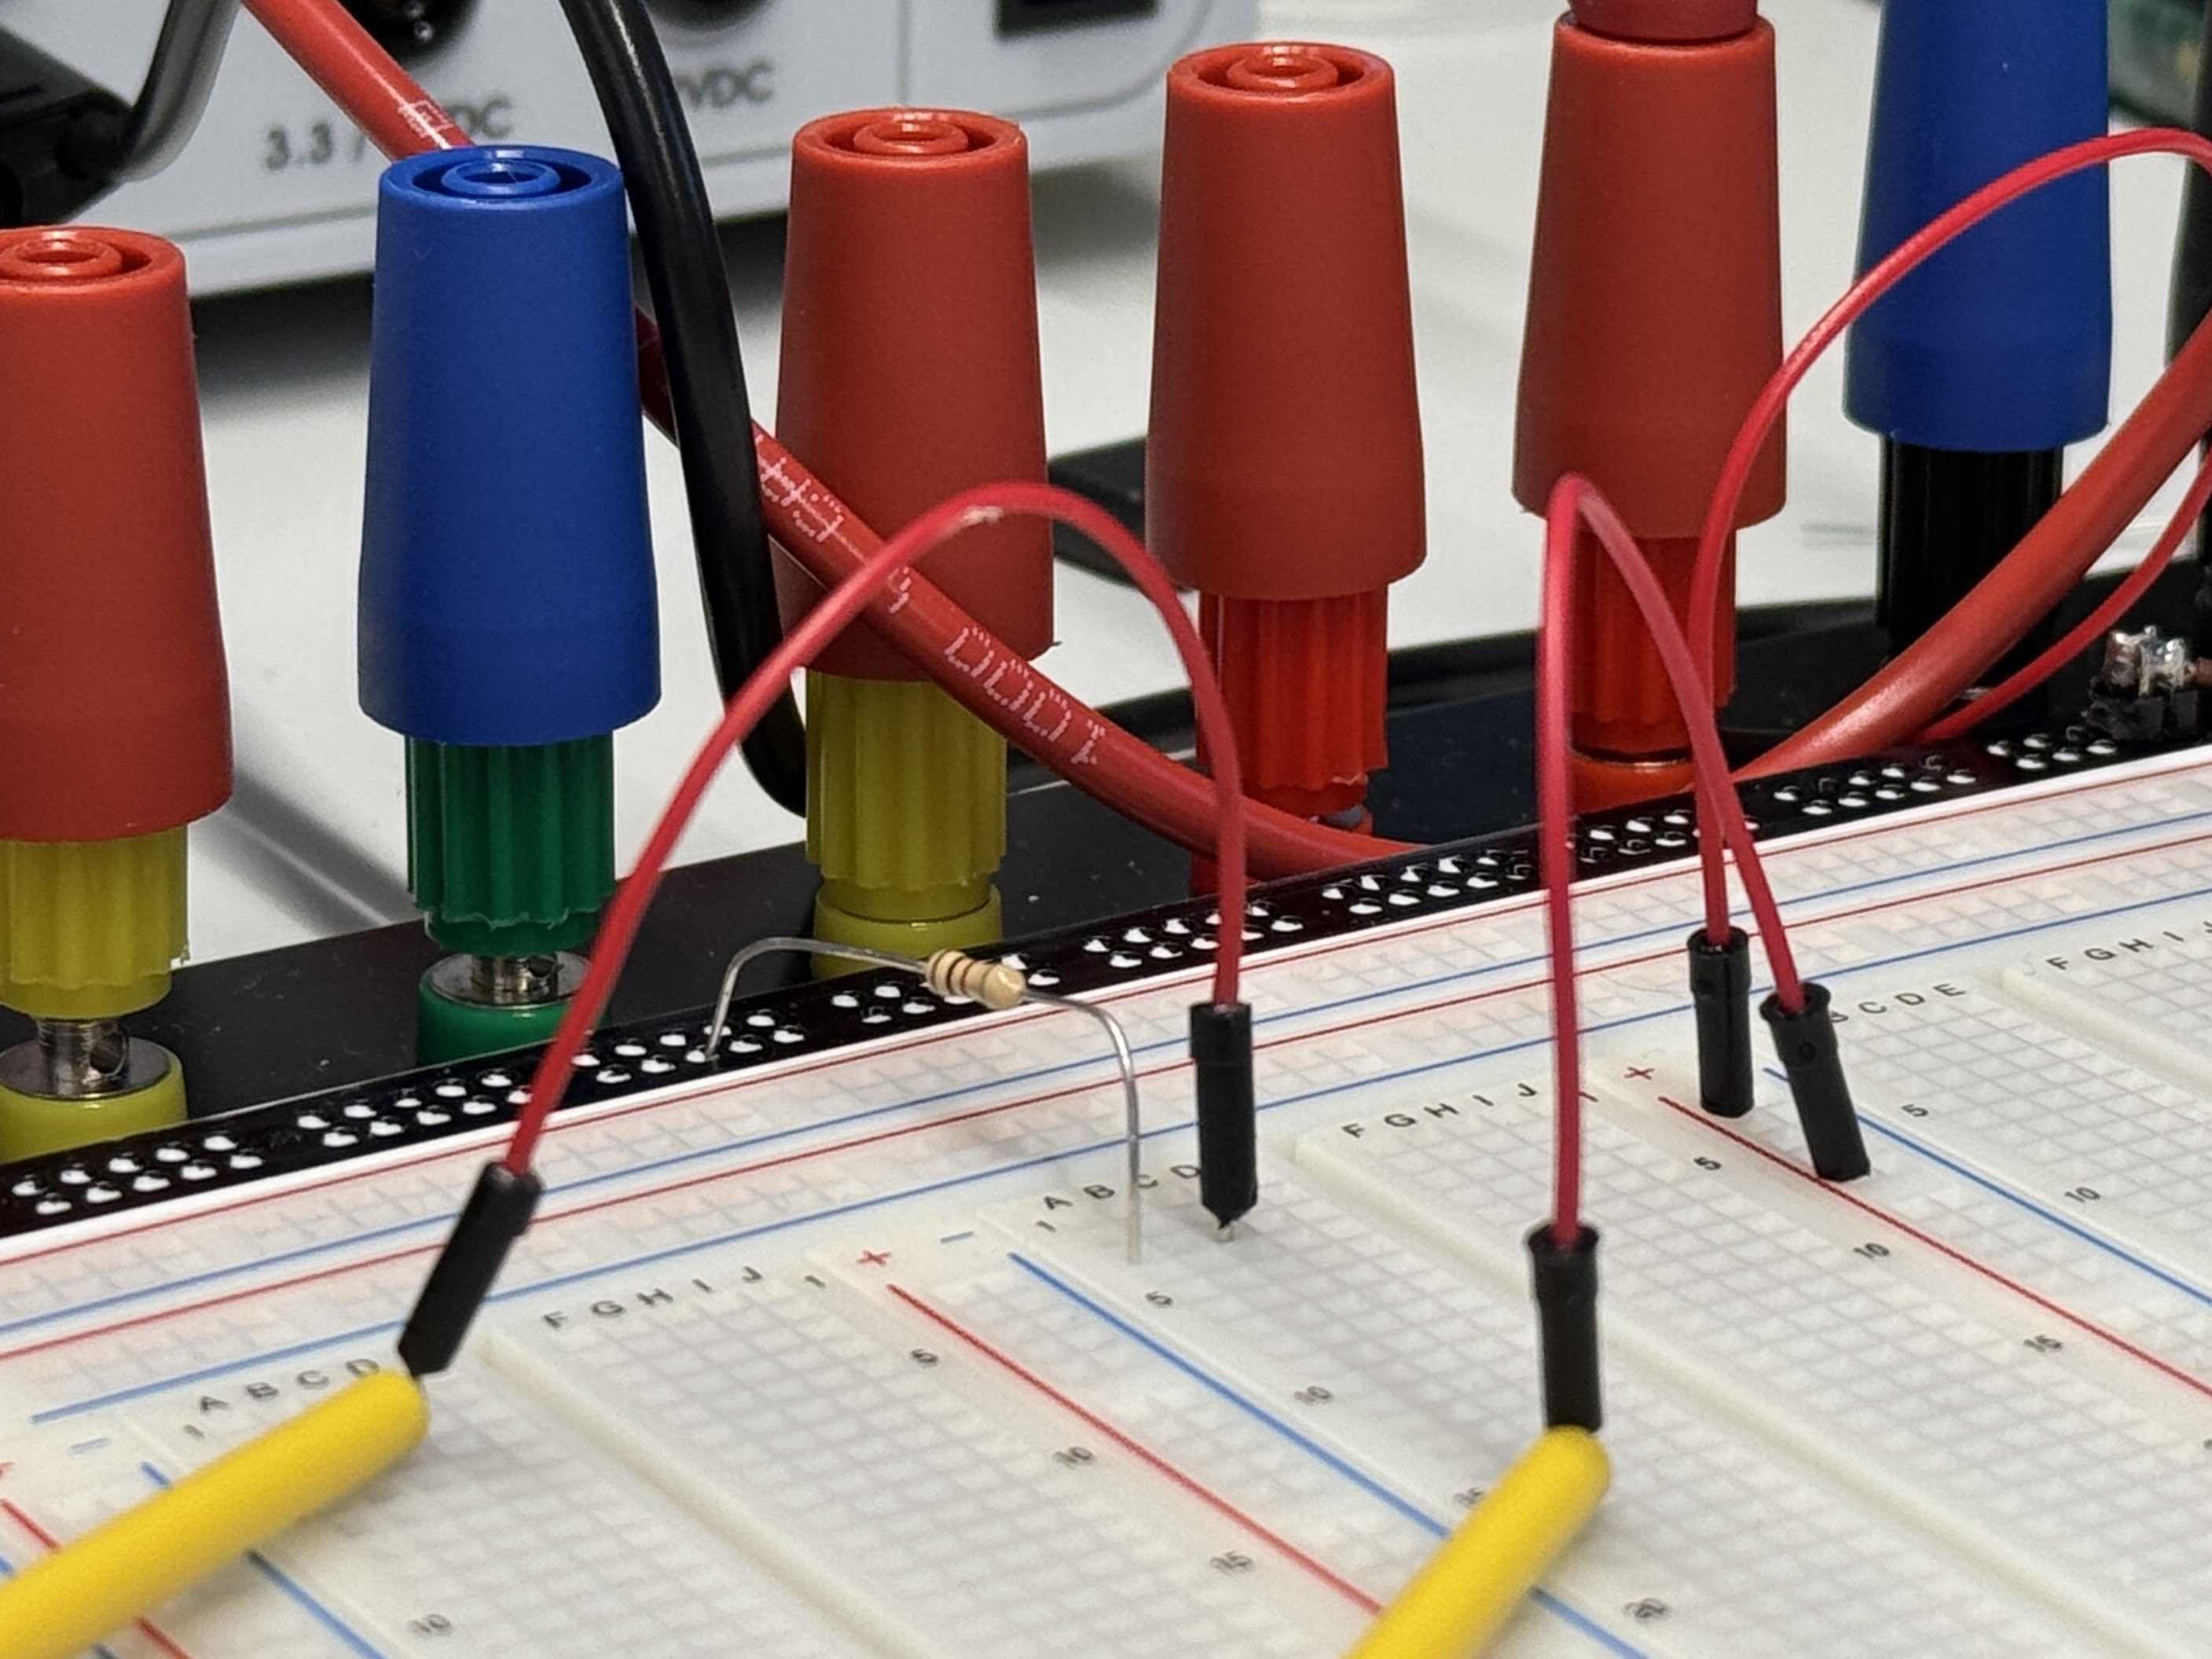
\includegraphics[width=0.8\textwidth]{../Quellen/Labor2/Fotos/IMG_3979.jpeg}
\caption{Messung R}
\end{figure}

\begin{figure}[H]
    \centering
    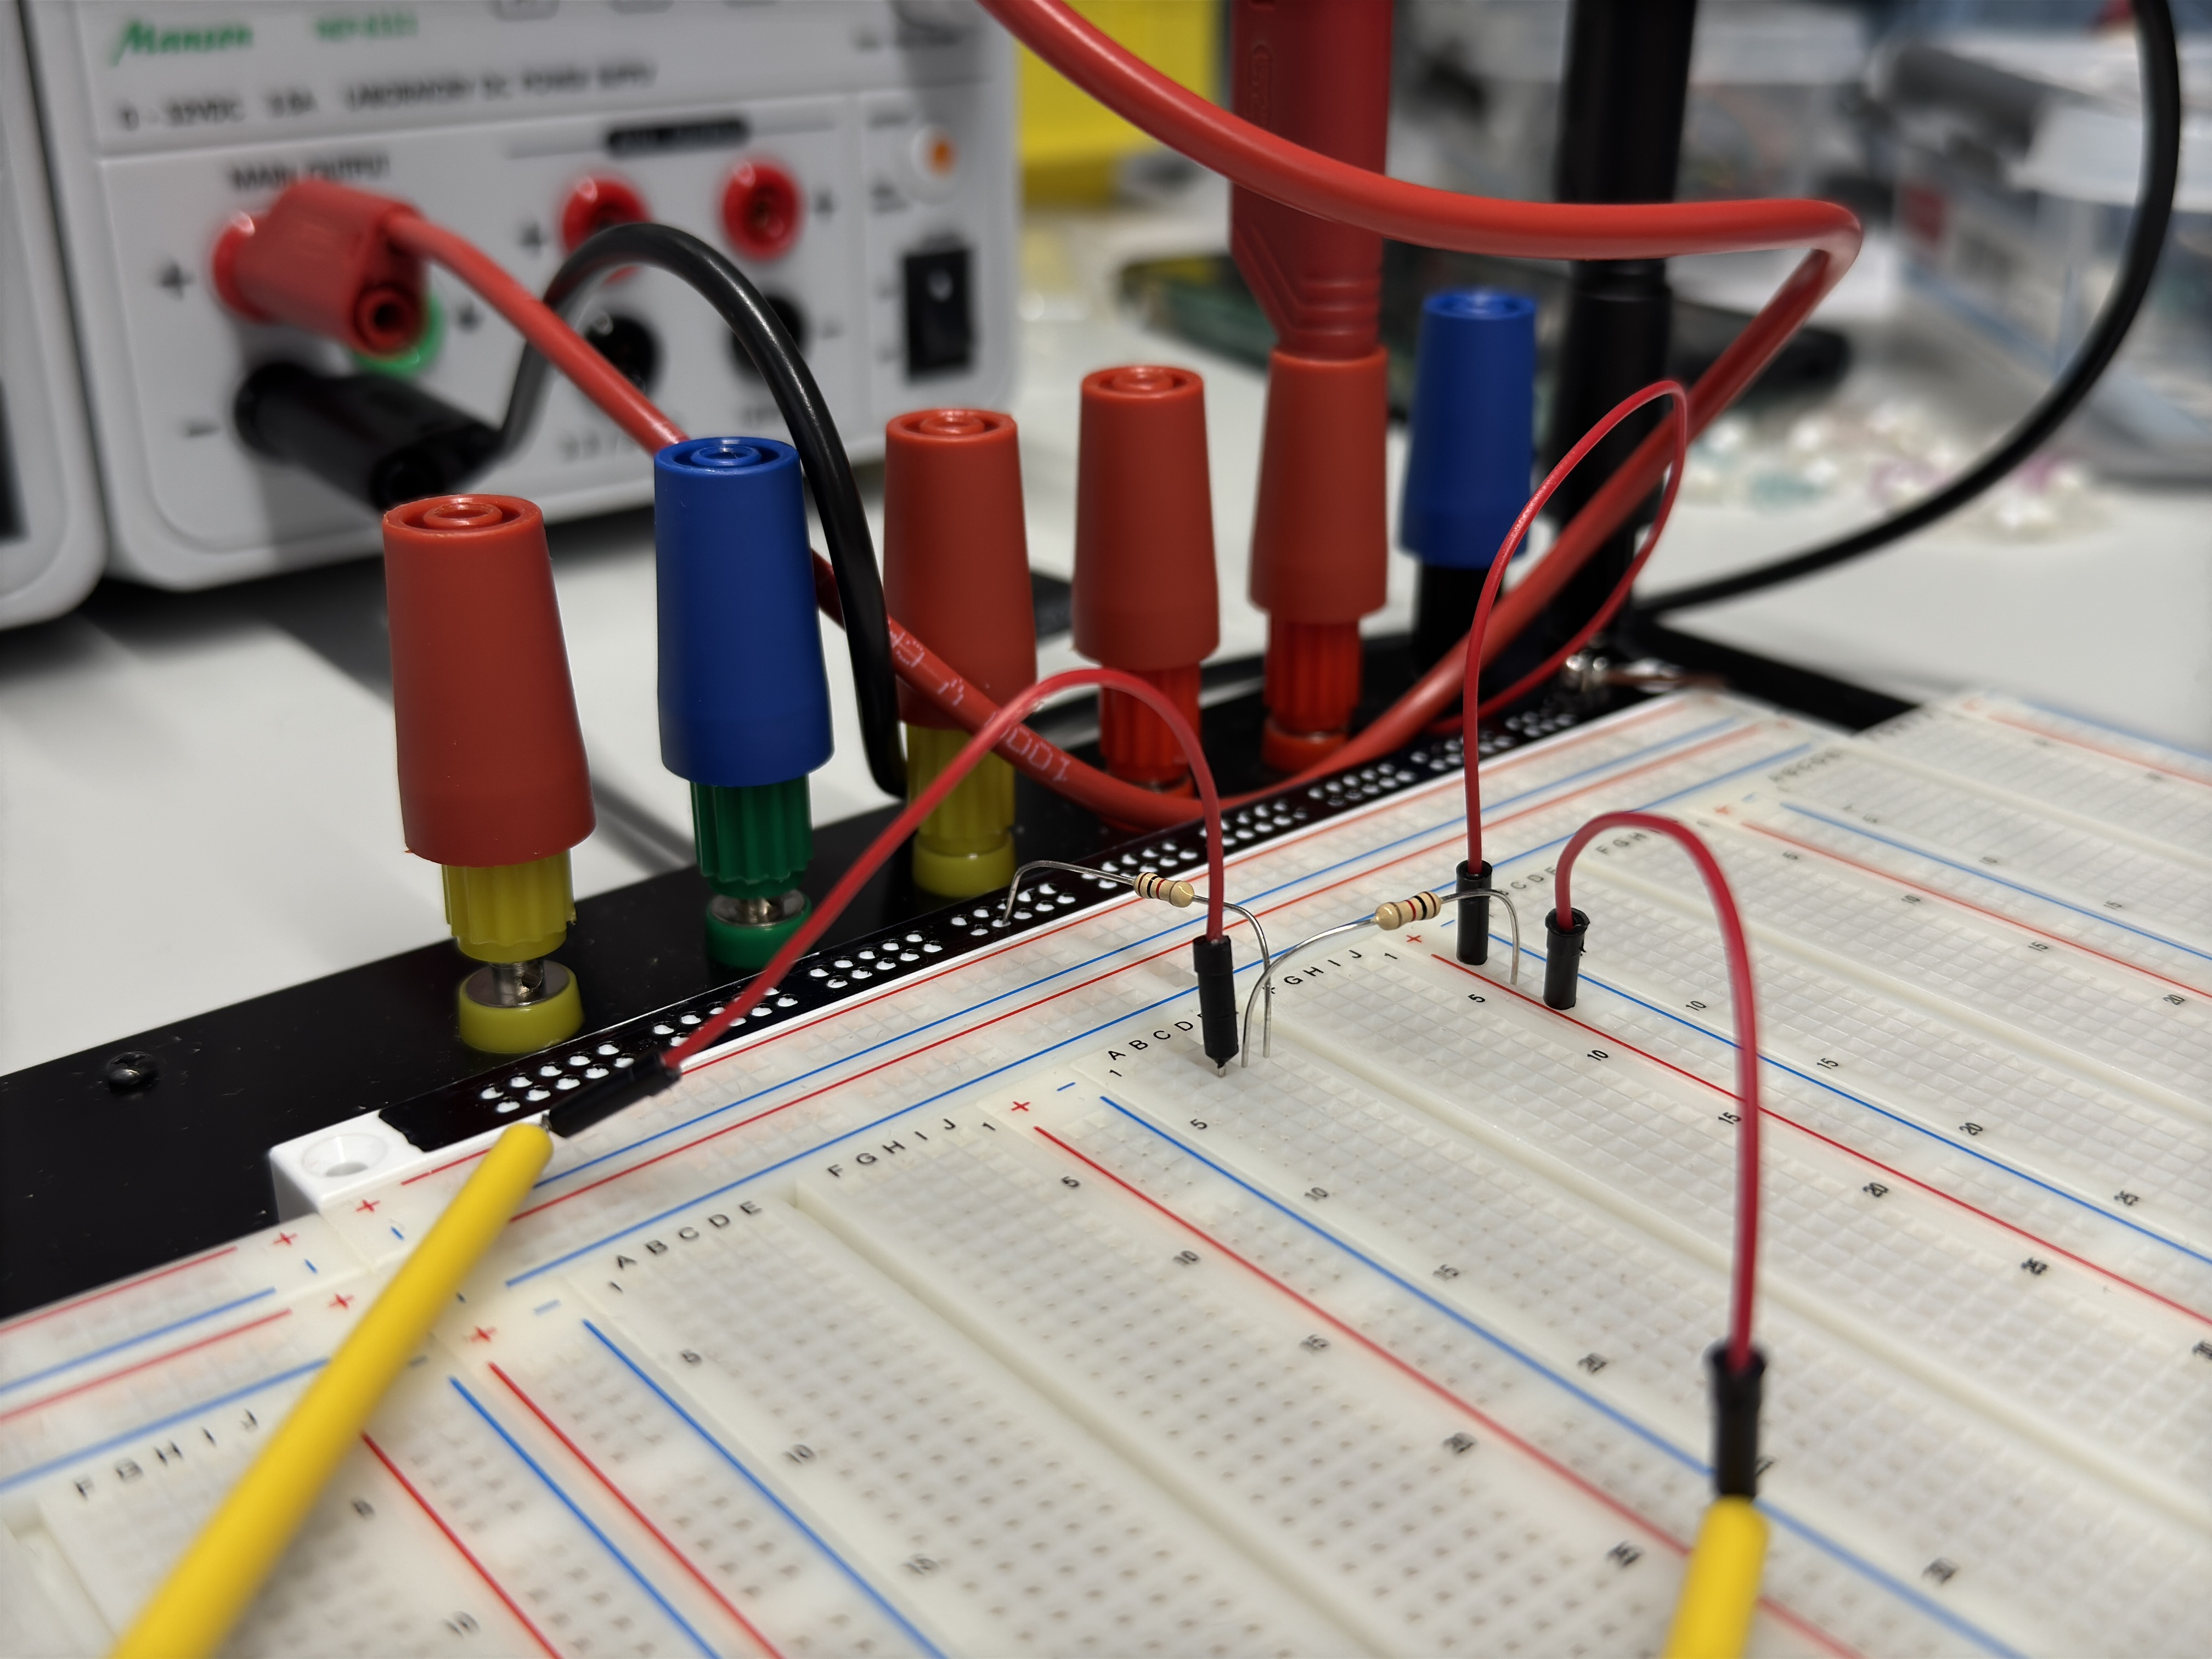
\includegraphics[width=0.8\textwidth]{../Quellen/Labor2/Fotos/IMG_3980.jpeg}
\caption{Messung R\textsubscript{v}}
\end{figure}


\subsection{Messergebnisse}
\begin{table}[H]
	\centering
	\begin{tabular}{|c|c|}
		\hline
		  & gemessener Widerstand\\
		\hline		
		\textbf{R} & 988 $\Omega$\\
		\hline
		\textbf{R\textsubscript{v}} & 996 $\Omega$\\
		\hline
	\end{tabular}
	\caption{Nachmessung der Widerstände}
\end{table}
!!!!!


\newpage
\section{Versuch 4: Widerstandsmessung mittels Vierdrahtmethode}
\subsection{Zielsetzung}
Es soll der (sehr niederohmige) Übergangswiderstand eines Kabels inklusive seiner Steckverbinder
mittels der Vierdrahtmethode gemessen werden. Der Fokus liegt darauf, möglichst Präzise den Widerstand des gesamten Kabels zu ermitteln, ohne die Werte mit der Messmethode zu verfälschen.

\subsection{Bauteile und Messgeräte}
\begin{itemize}
\item Labornetzgerät (NEP-8323)
\item Fluke 87 V True RMS Multimeter
\item Bananenkabel 2 Stück (Messobjekt und Messkabel)
\end{itemize}

\subsection{Messkonzept}
Das Messkonzept basiert auf der Nutzung der Vierdrahtmethode. Sie kann hohe Genauigkeit erzielen, was bei derart kleinen Widerständen, wie der eines Kabels, sehr von Vorteil ist. Im Detail wird der Messaufbau so realisiert, dass zwei separate Strom- und Spannungspfade verwendet werden. Dadurch, dass über die Messleitung kein Strom fließt, fällt dadurch dort nur sehr wenig Spannung ab und sie verfälscht so nicht den Widerstand.\\
\noindent Ein Multimeter hingegen würde den Messtrom über die Messleitung leiten und die dabei entstehenden Leitungswiderstände mitmessen. Diese parasitären Widerstände führen zu einer Verfälschung des Messergebnisses. \\\\
\noindent  {\bfseries Netzteil Einstellungen:\par}
\noindent Am Netzteil leuchtet die Anzeige für C.C (= Constant Current), was bedeutet, dass sich das Gerät im Konstantstrom Modus befindet und über Spannungsanpassungen den Strom konstant hält. Die Strombegrenzung in diesem Modus hat verschiedene Einflüsse:
\begin{itemize}
\item Zu niedrig: Spannungsabfall zu klein, um vom Messgerät präzise gemssen zu werden. Höhere Ströme erzeugen einen größeren Spannungsabfall, der leichter und genauer zu messen ist, insbesondere bei niederohmigen Widerständen.
\item Zu hoch: Messtrom erwärmt das Objekt, wodurch der Widerstand steigt und das Ergebnis verfälscht wird.
\item Zu hoch: Überlastung des Netzerätes, Abschaltung\\
\end{itemize}
\newpage
\noindent  {\bfseries Die Grenzen der Strombegrenzung:\par}
\begin{itemize}
\item Seitens des Netzgeräts: Das Netzteil verfügt über eine maximale Stromausgabe von 3,5 A.
\item Seitens der Anwendung: Die genauen Spezifikationen des Kabels sind unbekannt. Typischerweise können Bananenkabel diesen Durchmessers mit etwa 30 A belastet werden. 
\item Bei anderen Anwendungen: 
	\begin{itemize}
	\item Bauteilschutz: In Anwendungen, die Halbleiterbauteilen oder andere empfindlichen Bauteile beinhalten, darf der Strom bestimmte Bauteilgrenzen nicht überschreiten, um Zerstörung oder Funktionsbeeinträchtigungen zu verhindern.
	\item Effizienz: Ein zu hoher Strom führt generell zu Energieverlusten.\\
	\end{itemize}
\end{itemize}
\noindent  {\bfseries Aufbau der Messchaltung:\par}
\noindent Um den gesamten Widerstand des Kabels inklusiver seiner Steckverbindungen, wie er bei reellen Nutzungssituationen vorkommt, zu ermitteln, muss die Reihenfolge der Steckverbindungen beachtet werden. 

\begin{figure}[H]
    \centering
    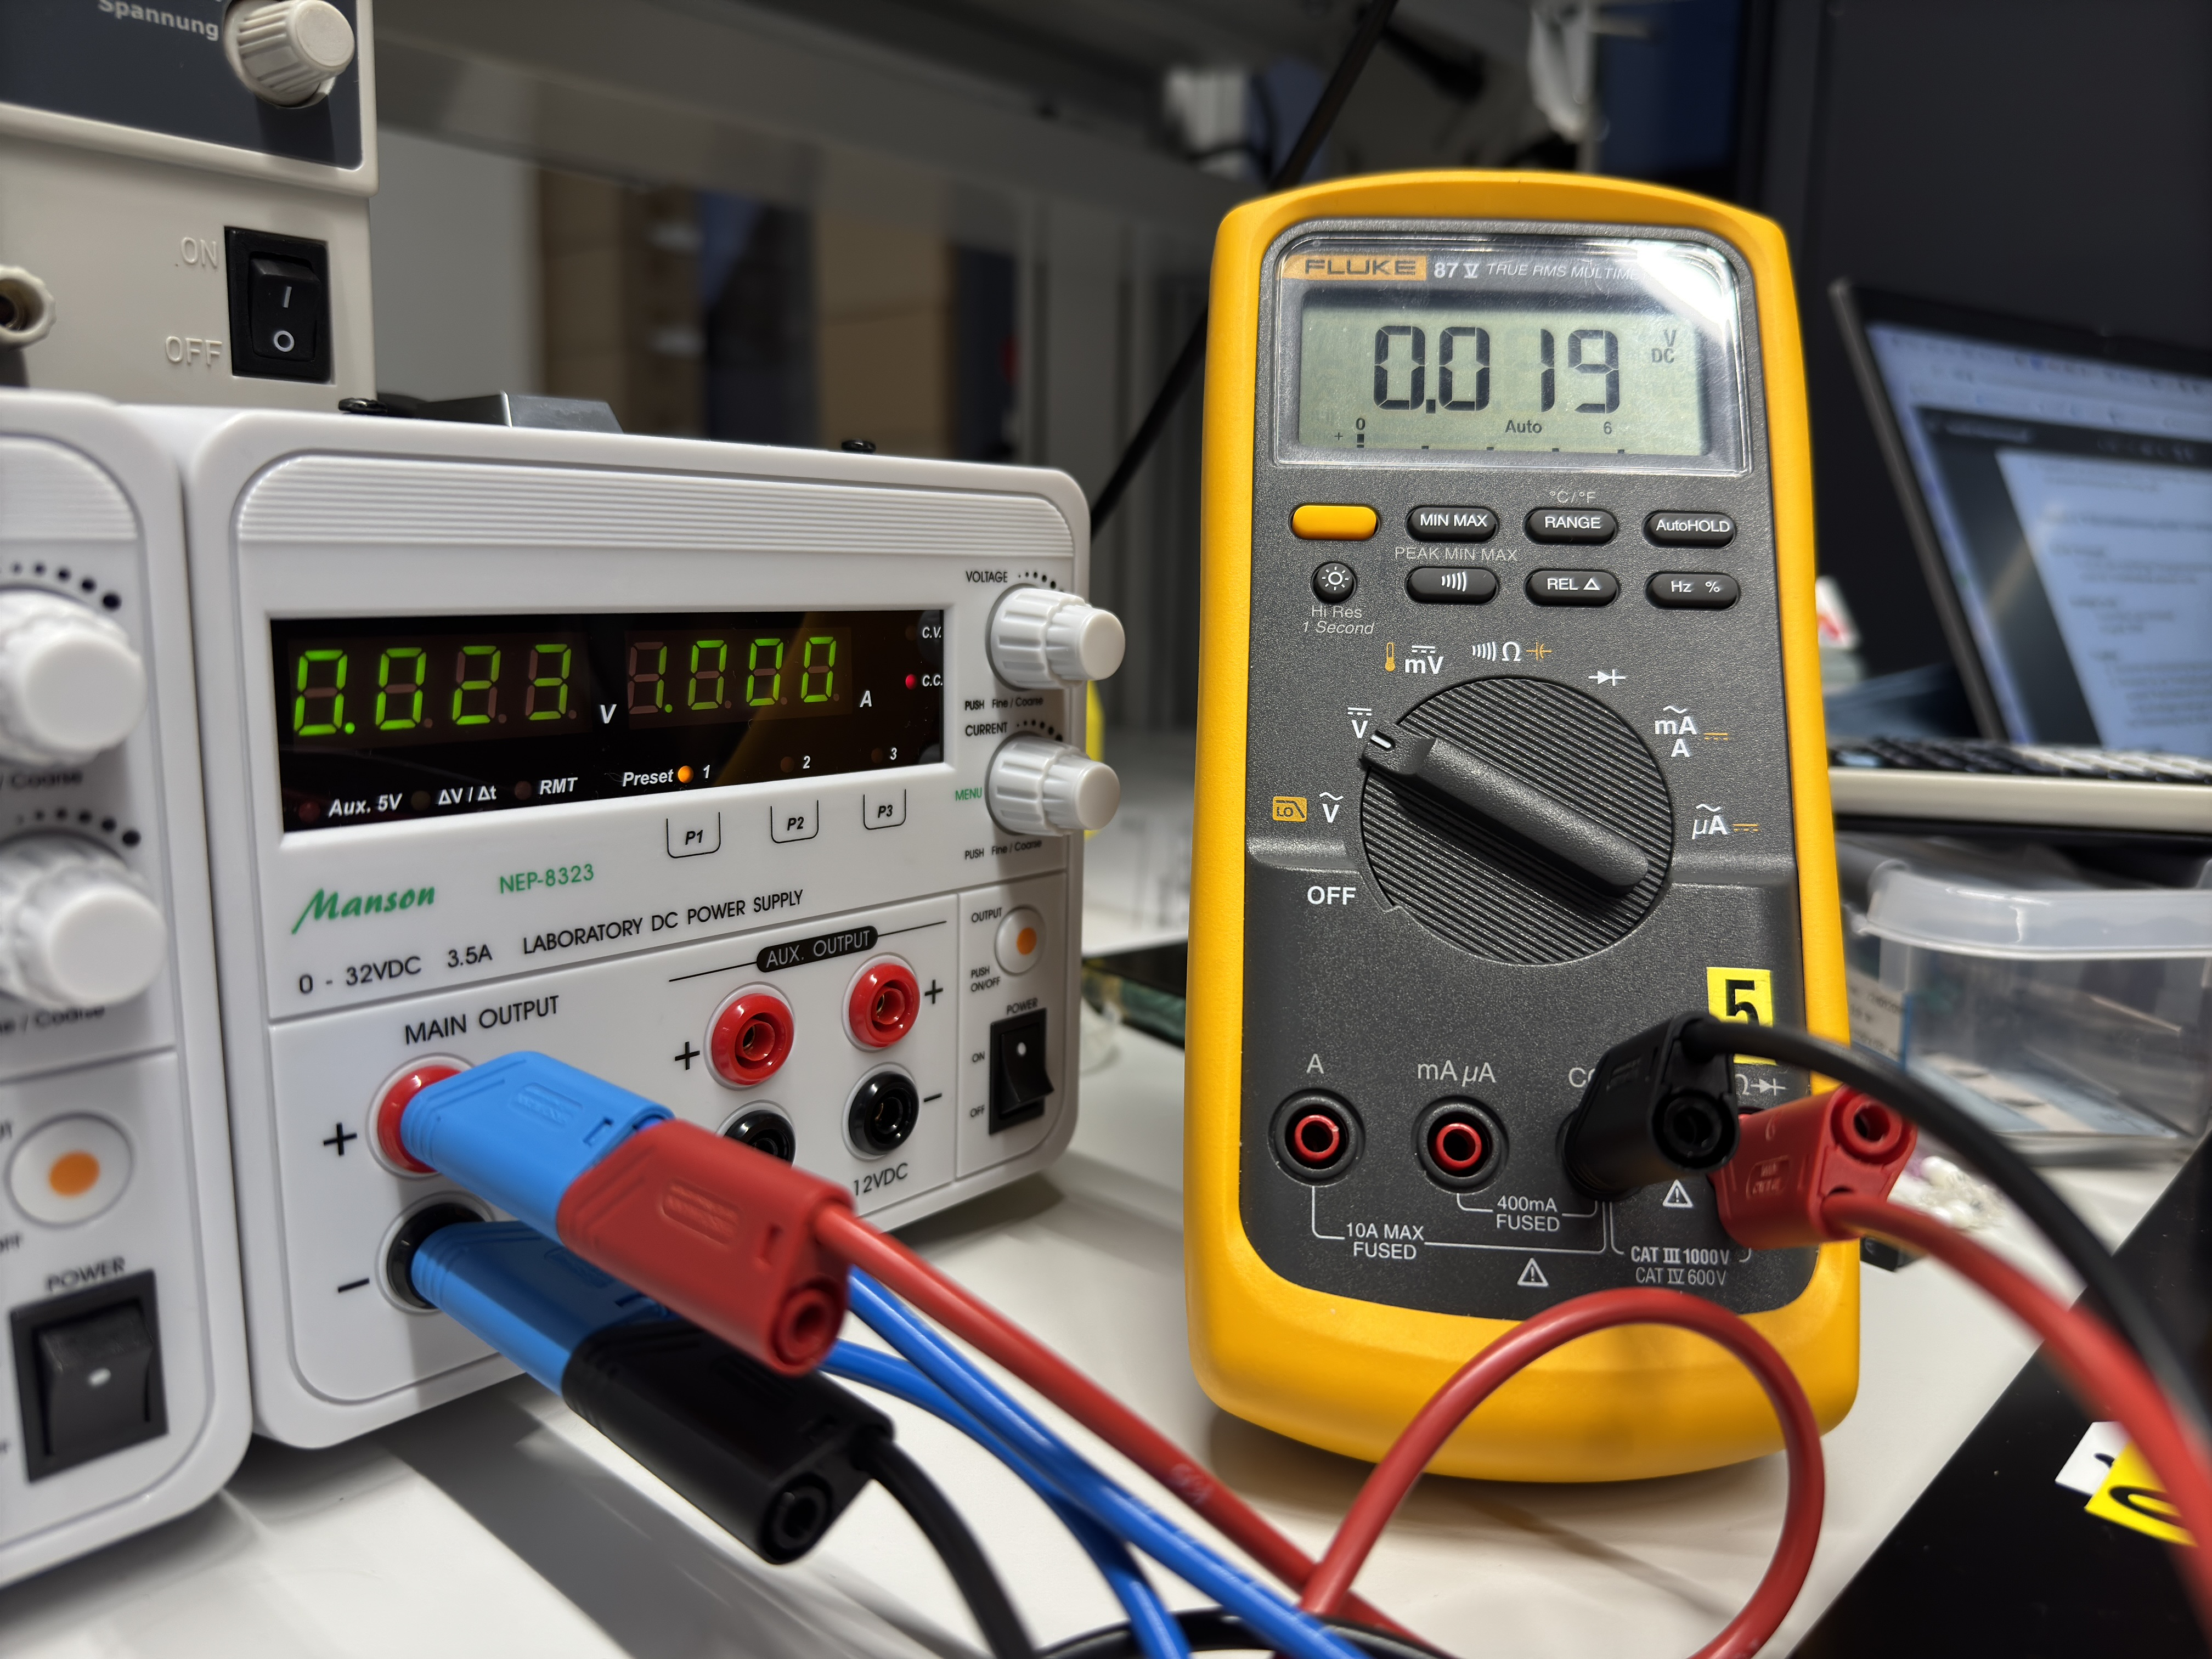
\includegraphics[width=1\textwidth]{../Quellen/Labor2/Fotos/IMG_3983.jpeg}
\caption{Teil der Steckverbindung nicht berücksichtigt}
\end{figure}

\begin{figure}[H]
    \centering
    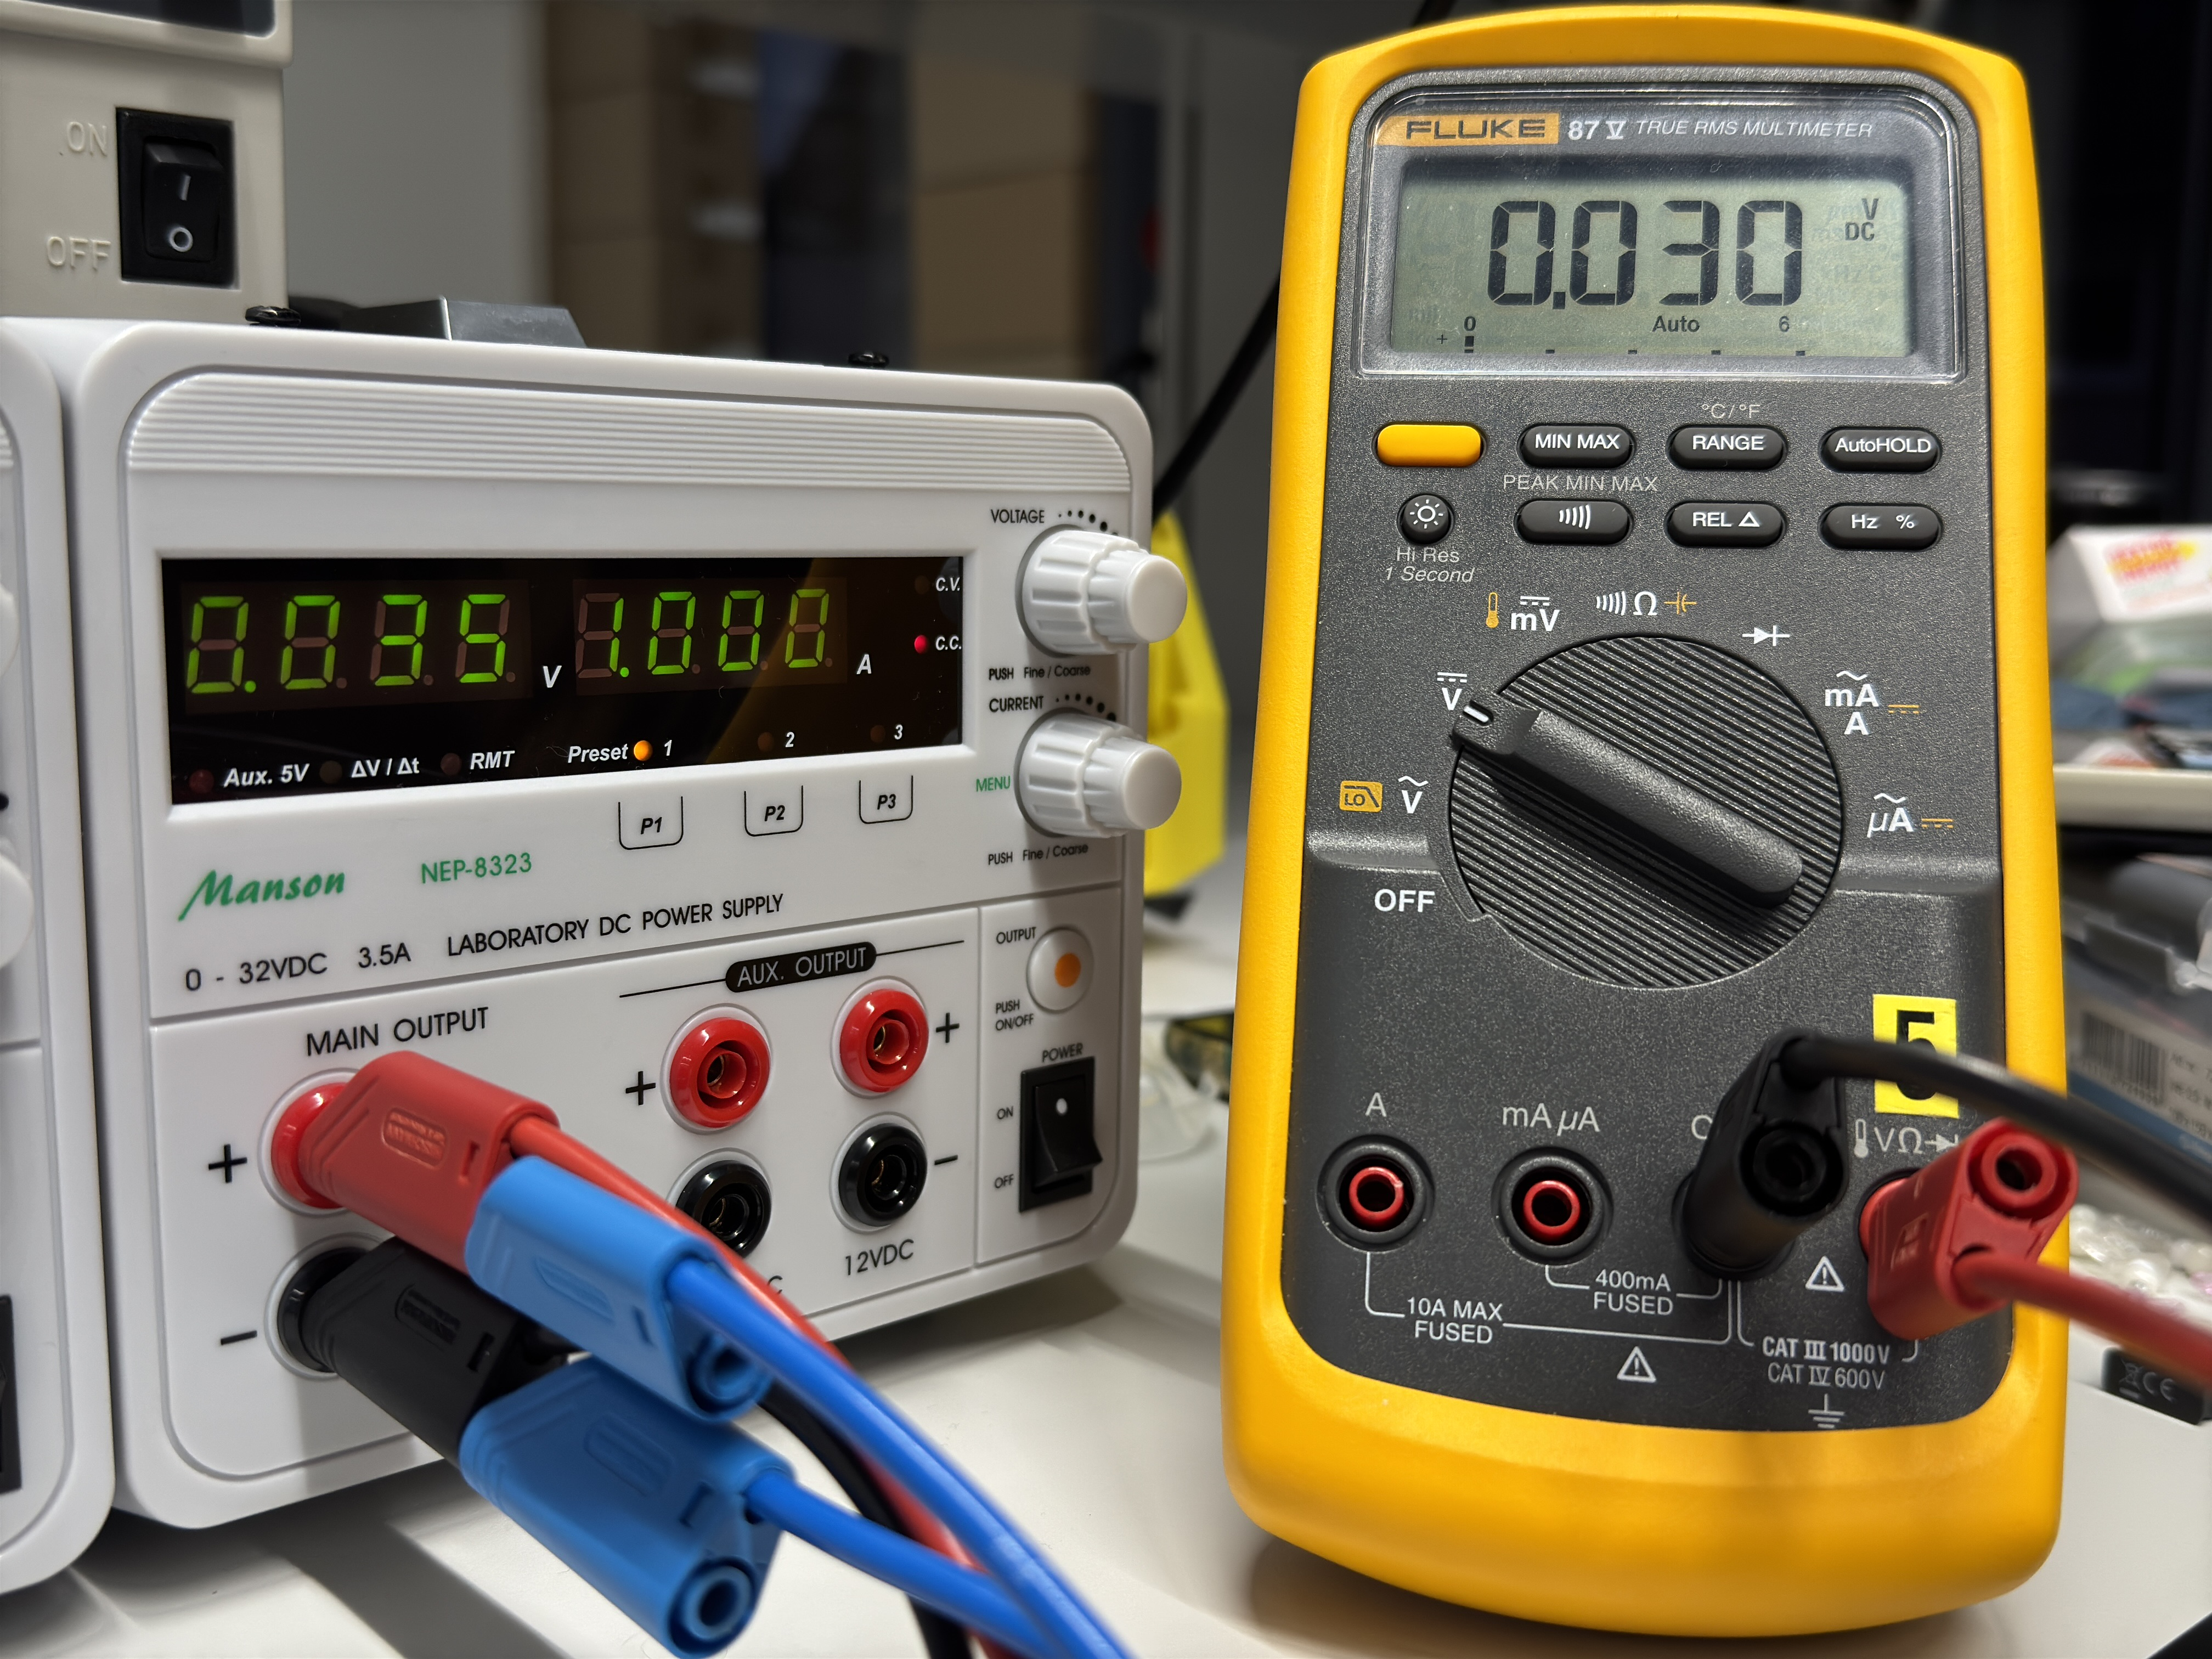
\includegraphics[width=1\textwidth]{../Quellen/Labor2/Fotos/IMG_3982.jpeg}
\caption{Messung über gesamtes Objekt inkl. der ganzen Steckverbindungen}
\end{figure}

\subsection{Messergebnisse}
Um den Widerstand des blauen Kabels zu berechnen, verwenden wir die Differenz der Spannungswerte zwischen dem Netzteil und dem Digitalmultimeter.\\\\
   - Spannung am Netzteil: \( U_{\text{Netzteil}} = 0,035 \, \text{V} \) \\
   - Spannung am DMM: \( U_{\text{DMM}} = 0,030 \, \text{V} \) \\
   - Strom durch das Kabel: \( I = 1,000 \, \text{A} \) \\\\
Spannungsabfall über das Kabel:
   \[
   \Delta U = U_{\text{Netzteil}} - U_{\text{DMM}} = 0,035 \, \text{V} - 0,030 \, \text{V} = 0,005 \, \text{V}
   \]\\
Berechnung des Widerstands:
   \[
   R = \frac{\Delta U}{I} = \frac{0,005 \, \text{V}}{1,000 \, \text{A}} = 0,005 \, \Omega
   \]

\newpage
\section{Versuch 5: Statistik}
\subsection{Zielsetzung}
Aufgabenstellung: Bestimmung einer gemessenen Zufallsverteilung und ihrer Eigenschaften (Momente). Hierbei stellt
das vorgegebene Los von Widerständen eine willkürlich entnommene Stichprobe einer vom
Hersteller erzeugten Grundgesamtheit dar.\\
\noindent Die Eigenschaften der gemessenen Zufallsverteilung zu bestimmen, insbesondere den Mittelwert und die empirische Standardabweichung. Diese Messung ermöglicht es, die Verteilung der Werte und die Toleranzen der Bauteile zu bewerten sowie zu untersuchen, inwieweit die gemessenen Ergebnisse mit den Herstellerangaben übereinstimmen.


\subsection{Bauteile und Messgeräte}
\begin{itemize}
\item Fluke 87 V True RMS Multimeter
\item Widerstandsgurt mit 25 Widerständen
\end{itemize}

\subsection{Messkonzept}
Am Fluke Multimeter wird die Widerstandsmessung aktiviert. Es ermöglicht die Messung einzelner Widerstände mithilfe von Klemmen, die ans Multimeter angeschlossen werden. Mit dem Widerstand wird ein geschlossener Stromkreis gebildet, in dem das Multimeter den Widerstand mithilfe eines kleinen Messtroms bestimmt.\\
\noindent Bei dieser Messung können die parasitären Widerstände der Kabel vernachlässigt werden, da sie im Vergleich zu den zu messenden Widerstandsbauteilen verschwindend gering sind.

\begin{figure}[H]
    \centering
    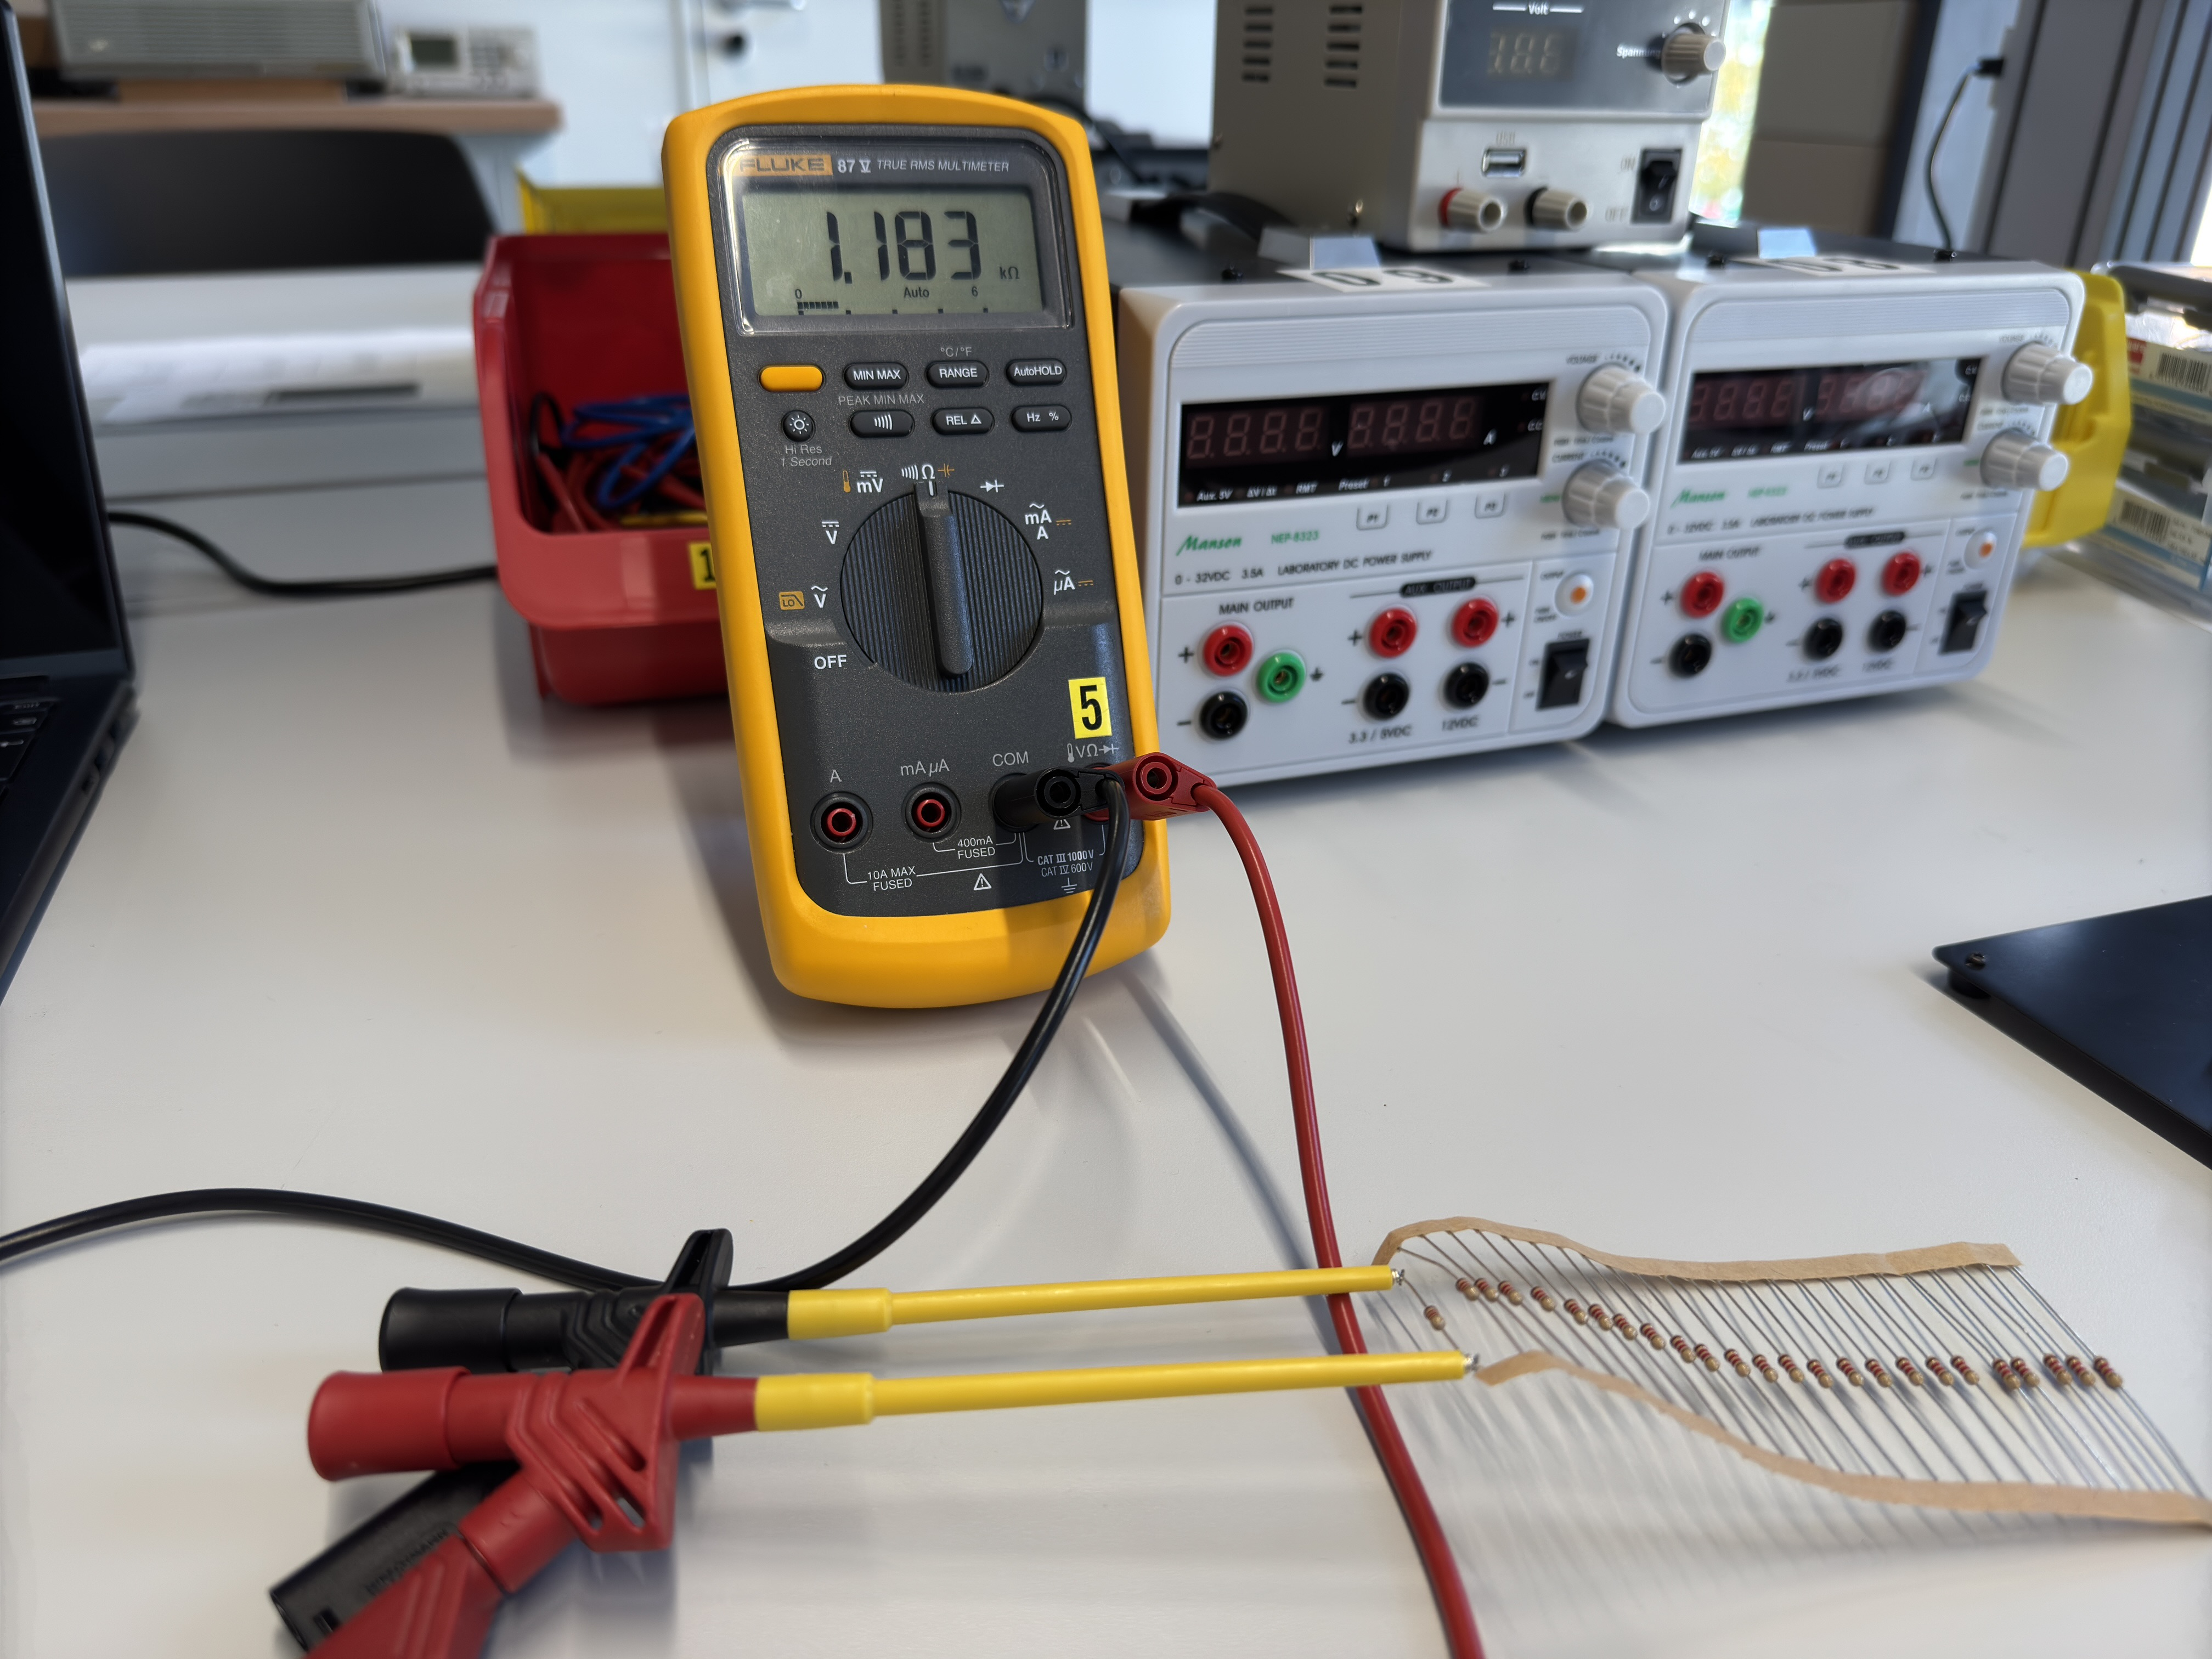
\includegraphics[width=0.85\textwidth]{../Quellen/Labor2/Fotos/IMG_4011.jpeg}
\caption{Messschaltung}
\end{figure}

\subsection{Messergebnisse}
\begin{table}[H]
	\centering
	\begin{tabular}{|c|c|c|c|}
		\hline
		Widerstand Nr. & Wert in kOhm & Widerstand Nr. & Wert in kOhm \\
		\hline
		1 & 1.183 & 14 & 1.183 \\
		2 & 1.181 & 15 & 1.180 \\
		3 & 1.186 & 16 & 1.183 \\
		4 & 1.181 & 17 & 1.180 \\
		5 & 1.186 & 18 & 1.182 \\
		6 & 1.183 & 19 & 1.184 \\
		7 & 1.182 & 20 & 1.183 \\
		8 & 1.181 & 21 & 1.184 \\
		9 & 1.187 & 22 & 1.187 \\
		10 & 1.181 & 23 & 1.182 \\
		11 & 1.188 & 24 & 1.179 \\
		12 & 1.186 & 25 & 1.187 \\
		13 & 1.179 & - & - \\
		\hline
	\end{tabular}
	\caption{Einzelne Messungen}
\end{table}

\begin{figure}[H]
    \centering
    \includegraphics[width=0.85\textwidth]{../Quellen/Labor2/Histogramm-Widerstände.png}
\caption{Histogramm}
\end{figure}

Der Mittelwert \( \bar{x} \) wird berechnet als:
\[
\bar{x} = \frac{1}{n} \sum_{i=1}^{n} x_i
\]
\[
\bar{x} = \frac{29.582}{25} = 1.1833 \, \text{k}\Omega
\]

Die empirische Standardabweichung \( s \) wird berechnet als:
\[
s = \sqrt{\frac{1}{n-1} \sum_{i=1}^{n} (x_i - \bar{x})^2}
\]

\textbf{Berechnung der Abweichungen:}
\[
x_i - \bar{x} \quad \text{für jeden Messwert}:
\]
Beispiele: 
\[
1.183 - 1.1833 = -0.0003, \quad 1.181 - 1.1833 = -0.0023, \quad \dots
\]

\textbf{Quadratische Abweichungen:}
\[
(x_i - \bar{x})^2 \quad \text{für jeden Messwert}:
\]
Beispiele:
\[
(-0.0003)^2 = 9 \times 10^{-8}, \quad (-0.0023)^2 = 5.29 \times 10^{-6}, \quad \dots
\]

\textbf{Summe der quadratischen Abweichungen:}
\[
\sum_{i=1}^{n} (x_i - \bar{x})^2 = 0.000192
\]

\textbf{Einsetzen in die Formel:}
\[
s = \sqrt{\frac{0.000192}{25 - 1}} = \sqrt{\frac{0.000192}{24}} = \sqrt{0.000008} = 0.0028 \, \text{k}\Omega
\]
\section*{Vergleich der invertierenden und nicht-invertierenden Grundschaltung eines Operationsverstärkers}

\subsection*{1. Allgemeine Spannungsverstärkung}
\textbf{Invertierende Schaltung:}
\[
A_V = -\frac{R_f}{R_{in}}
\]
wobei:
\begin{itemize}
    \item \( R_f \) der Gegenkopplungswiderstand ist
    \item \( R_{in} \) der Eingangswiderstand ist
\end{itemize}

\textbf{Nicht-invertierende Schaltung:}
\[
A_V = 1 + \frac{R_f}{R_{in}}
\]
wobei:
\begin{itemize}
    \item \( R_f \) der Gegenkopplungswiderstand ist
    \item \( R_{in} \) der Widerstand zwischen Masse und dem invertierenden Eingang des Operationsverstärkers
\end{itemize}

\subsection*{2. Relative Verstärkungsänderung}
Angenommen, der Gegenkopplungswiderstand \( R_f \) wird durch einen Wert \( R_f + \Delta R_f \) ersetzt, wobei \( \Delta R_f \) die Abweichung aufgrund der Toleranz ist.

\textbf{Invertierende Schaltung:}
\[
A_V' = -\frac{R_f + \Delta R_f}{R_{in}}
\]
Die relative Verstärkungsänderung \( \frac{\Delta A_V}{A_V} \) ist:
\[
\frac{\Delta A_V}{A_V} = \frac{A_V' - A_V}{A_V} = \frac{\left( -\frac{R_f + \Delta R_f}{R_{in}} \right) - \left( -\frac{R_f}{R_{in}} \right)}{-\frac{R_f}{R_{in}}}
\]
Vereinfachung:
\[
\frac{\Delta A_V}{A_V} = \frac{\Delta R_f}{R_f}
\]

\textbf{Nicht-invertierende Schaltung:}
\[
A_V' = 1 + \frac{R_f + \Delta R_f}{R_{in}}
\]
Die relative Verstärkungsänderung \( \frac{\Delta A_V}{A_V} \) ist:
\[
\frac{\Delta A_V}{A_V} = \frac{A_V' - A_V}{A_V} = \frac{\left( 1 + \frac{R_f + \Delta R_f}{R_{in}} \right) - \left( 1 + \frac{R_f}{R_{in}} \right)}{1 + \frac{R_f}{R_{in}}}
\]
Vereinfachung:
\[
\frac{\Delta A_V}{A_V} = \frac{\frac{\Delta R_f}{R_{in}}}{1 + \frac{R_f}{R_{in}}}
\]

\subsection*{3. Empfindlichkeit der Schaltungen}
Die \textbf{invertierende Schaltung} ist proportional zur relativen Änderung \( \frac{\Delta R_f}{R_f} \), was bedeutet, dass die Verstärkungsänderung direkt von der Änderung des Gegenkopplungswiderstands abhängt.

Die \textbf{nicht-invertierende Schaltung} ist weniger empfindlich, da die Verstärkungsänderung durch den Faktor \( 1 + \frac{R_f}{R_{in}} \) abgeschwächt wird.

\textbf{Fazit:} Die invertierende Schaltung reagiert empfindlicher auf Änderungen des Gegenkopplungswiderstands.

\subsection*{4. Zahlenbeispiel}
Gegeben:
\begin{itemize}
    \item \( R_f = 10 \, \text{k}\Omega \)
    \item \( R_{in} = 1 \, \text{k}\Omega \)
    \item Toleranz \( \Delta R_f = 5\% \), also \( \Delta R_f = 0,05 \times 10 \, \text{k}\Omega = 0,5 \, \text{k}\Omega \)
\end{itemize}

\textbf{Invertierende Schaltung:}
\[
\frac{\Delta A_V}{A_V} = \frac{\Delta R_f}{R_f} = \frac{0,5}{10} = 0,05 \quad \text{(5\% relative Änderung)}
\]

\textbf{Nicht-invertierende Schaltung:}
\[
\frac{\Delta A_V}{A_V} = \frac{\frac{\Delta R_f}{R_{in}}}{1 + \frac{R_f}{R_{in}}} = \frac{\frac{0,5}{1}}{1 + \frac{10}{1}} = \frac{0,5}{11} \approx 0,0455 \quad \text{(4,55\% relative Änderung)}
\]

\noindent Hier zeigt sich, dass die nicht-invertierende Schaltung eine geringere relative Verstärkungsänderung aufweist.


\section{Versuch 6: Aktiver Tiefpass erster Ordnung}
\subsection{Zielsetzung}
Bestimmung der frequenzabhängigen Verstärkung eines aktiven Tiefpasses

\subsection{Bauteile und Messgeräte}
\begin{itemize}
\item Netzgerät (NEP-8323)
\item Fluke 87 V True RMS Multimeter
\item Keysight Oszilloskop (DSOX1102A)
\item Bananenkabel (mehrere: rot, blau, schwarz)
\item Sicherheits-Klemmprüfspitze (2 Stück)
\item Oszilloskop BNC Tastkopf mit Messeklemme
\item Steckkabel (mehrere: im Idealfall verschiedene Farben)
\item Steckbrett\\
\end{itemize}


\begin{itemize}
\item A/D Converter - ADC080x
\item 10 Segment LED-Bar - OSX10201-B
\newpage
\item Kondensatoren: 
	\begin{itemize}
	\item 10 µF "Tantalum"
	\item 0,1 µF (2 Stück)
	\item 150 pF
	\end{itemize}
\item Widerstände: 
	\begin{itemize}
	\item 1k$\Omega$
	\item 10k$\Omega$
	\item 8 x 1 k$\Omega$ Widerstandsnetzwerk
	\end{itemize}
\end{itemize}

\subsection{Messkonzept}
...

\begin{figure}[H]
    \centering
 %   \includegraphics[]{}
\caption{...}
\end{figure}


\subsection{Messergebnisse}
...




\section{Diskussion}
Was würden Sie nächstes Mal anders machen? Was hat besondere Schwierigkeiten bereitet?

\end{document}
